\documentclass[]{book}
\usepackage{lmodern}
\usepackage{amssymb,amsmath}
\usepackage{ifxetex,ifluatex}
\usepackage{fixltx2e} % provides \textsubscript
\ifnum 0\ifxetex 1\fi\ifluatex 1\fi=0 % if pdftex
  \usepackage[T1]{fontenc}
  \usepackage[utf8]{inputenc}
\else % if luatex or xelatex
  \ifxetex
    \usepackage{mathspec}
  \else
    \usepackage{fontspec}
  \fi
  \defaultfontfeatures{Ligatures=TeX,Scale=MatchLowercase}
\fi
% use upquote if available, for straight quotes in verbatim environments
\IfFileExists{upquote.sty}{\usepackage{upquote}}{}
% use microtype if available
\IfFileExists{microtype.sty}{%
\usepackage{microtype}
\UseMicrotypeSet[protrusion]{basicmath} % disable protrusion for tt fonts
}{}
\usepackage[margin=1in]{geometry}
\usepackage{hyperref}
\hypersetup{unicode=true,
            pdftitle={BIO 4022. Manipulación de datos e investigación reproducible en R},
            pdfauthor={Derek Corcoran},
            pdfborder={0 0 0},
            breaklinks=true}
\urlstyle{same}  % don't use monospace font for urls
\usepackage{natbib}
\bibliographystyle{apalike}
\usepackage{color}
\usepackage{fancyvrb}
\newcommand{\VerbBar}{|}
\newcommand{\VERB}{\Verb[commandchars=\\\{\}]}
\DefineVerbatimEnvironment{Highlighting}{Verbatim}{commandchars=\\\{\}}
% Add ',fontsize=\small' for more characters per line
\usepackage{framed}
\definecolor{shadecolor}{RGB}{248,248,248}
\newenvironment{Shaded}{\begin{snugshade}}{\end{snugshade}}
\newcommand{\AlertTok}[1]{\textcolor[rgb]{0.94,0.16,0.16}{#1}}
\newcommand{\AnnotationTok}[1]{\textcolor[rgb]{0.56,0.35,0.01}{\textbf{\textit{#1}}}}
\newcommand{\AttributeTok}[1]{\textcolor[rgb]{0.77,0.63,0.00}{#1}}
\newcommand{\BaseNTok}[1]{\textcolor[rgb]{0.00,0.00,0.81}{#1}}
\newcommand{\BuiltInTok}[1]{#1}
\newcommand{\CharTok}[1]{\textcolor[rgb]{0.31,0.60,0.02}{#1}}
\newcommand{\CommentTok}[1]{\textcolor[rgb]{0.56,0.35,0.01}{\textit{#1}}}
\newcommand{\CommentVarTok}[1]{\textcolor[rgb]{0.56,0.35,0.01}{\textbf{\textit{#1}}}}
\newcommand{\ConstantTok}[1]{\textcolor[rgb]{0.00,0.00,0.00}{#1}}
\newcommand{\ControlFlowTok}[1]{\textcolor[rgb]{0.13,0.29,0.53}{\textbf{#1}}}
\newcommand{\DataTypeTok}[1]{\textcolor[rgb]{0.13,0.29,0.53}{#1}}
\newcommand{\DecValTok}[1]{\textcolor[rgb]{0.00,0.00,0.81}{#1}}
\newcommand{\DocumentationTok}[1]{\textcolor[rgb]{0.56,0.35,0.01}{\textbf{\textit{#1}}}}
\newcommand{\ErrorTok}[1]{\textcolor[rgb]{0.64,0.00,0.00}{\textbf{#1}}}
\newcommand{\ExtensionTok}[1]{#1}
\newcommand{\FloatTok}[1]{\textcolor[rgb]{0.00,0.00,0.81}{#1}}
\newcommand{\FunctionTok}[1]{\textcolor[rgb]{0.00,0.00,0.00}{#1}}
\newcommand{\ImportTok}[1]{#1}
\newcommand{\InformationTok}[1]{\textcolor[rgb]{0.56,0.35,0.01}{\textbf{\textit{#1}}}}
\newcommand{\KeywordTok}[1]{\textcolor[rgb]{0.13,0.29,0.53}{\textbf{#1}}}
\newcommand{\NormalTok}[1]{#1}
\newcommand{\OperatorTok}[1]{\textcolor[rgb]{0.81,0.36,0.00}{\textbf{#1}}}
\newcommand{\OtherTok}[1]{\textcolor[rgb]{0.56,0.35,0.01}{#1}}
\newcommand{\PreprocessorTok}[1]{\textcolor[rgb]{0.56,0.35,0.01}{\textit{#1}}}
\newcommand{\RegionMarkerTok}[1]{#1}
\newcommand{\SpecialCharTok}[1]{\textcolor[rgb]{0.00,0.00,0.00}{#1}}
\newcommand{\SpecialStringTok}[1]{\textcolor[rgb]{0.31,0.60,0.02}{#1}}
\newcommand{\StringTok}[1]{\textcolor[rgb]{0.31,0.60,0.02}{#1}}
\newcommand{\VariableTok}[1]{\textcolor[rgb]{0.00,0.00,0.00}{#1}}
\newcommand{\VerbatimStringTok}[1]{\textcolor[rgb]{0.31,0.60,0.02}{#1}}
\newcommand{\WarningTok}[1]{\textcolor[rgb]{0.56,0.35,0.01}{\textbf{\textit{#1}}}}
\usepackage{longtable,booktabs}
\usepackage{graphicx,grffile}
\makeatletter
\def\maxwidth{\ifdim\Gin@nat@width>\linewidth\linewidth\else\Gin@nat@width\fi}
\def\maxheight{\ifdim\Gin@nat@height>\textheight\textheight\else\Gin@nat@height\fi}
\makeatother
% Scale images if necessary, so that they will not overflow the page
% margins by default, and it is still possible to overwrite the defaults
% using explicit options in \includegraphics[width, height, ...]{}
\setkeys{Gin}{width=\maxwidth,height=\maxheight,keepaspectratio}
\IfFileExists{parskip.sty}{%
\usepackage{parskip}
}{% else
\setlength{\parindent}{0pt}
\setlength{\parskip}{6pt plus 2pt minus 1pt}
}
\setlength{\emergencystretch}{3em}  % prevent overfull lines
\providecommand{\tightlist}{%
  \setlength{\itemsep}{0pt}\setlength{\parskip}{0pt}}
\setcounter{secnumdepth}{5}
% Redefines (sub)paragraphs to behave more like sections
\ifx\paragraph\undefined\else
\let\oldparagraph\paragraph
\renewcommand{\paragraph}[1]{\oldparagraph{#1}\mbox{}}
\fi
\ifx\subparagraph\undefined\else
\let\oldsubparagraph\subparagraph
\renewcommand{\subparagraph}[1]{\oldsubparagraph{#1}\mbox{}}
\fi

%%% Use protect on footnotes to avoid problems with footnotes in titles
\let\rmarkdownfootnote\footnote%
\def\footnote{\protect\rmarkdownfootnote}

%%% Change title format to be more compact
\usepackage{titling}

% Create subtitle command for use in maketitle
\newcommand{\subtitle}[1]{
  \posttitle{
    \begin{center}\large#1\end{center}
    }
}

\setlength{\droptitle}{-2em}

  \title{BIO 4022. Manipulación de datos e investigación reproducible en R}
    \pretitle{\vspace{\droptitle}\centering\huge}
  \posttitle{\par}
    \author{Derek Corcoran}
    \preauthor{\centering\large\emph}
  \postauthor{\par}
      \predate{\centering\large\emph}
  \postdate{\par}
    \date{2018-08-09}

\usepackage{booktabs}

\begin{document}
\maketitle

{
\setcounter{tocdepth}{1}
\tableofcontents
}
\hypertarget{parte-i}{%
\chapter*{Parte I}\label{parte-i}}
\addcontentsline{toc}{chapter}{Parte I}

\hypertarget{requerimientos}{%
\chapter*{Requerimientos}\label{requerimientos}}
\addcontentsline{toc}{chapter}{Requerimientos}

Para comenzar el trabajo se necesita la última versión de R y RStudio
\citep{R-base}.También se requiere de los paquetes \emph{pacman},
\emph{rmarkdown}, \emph{tidyverse} y \emph{tinytex}. Si no se ha usado R
o RStudio anteriormente, el siguiente video muestra cómo instalar ambos
programas y los paquetes necesarios para este curso en el siguiente
\href{https://youtu.be/RtkCAKXsVbw}{link}.

El código para la instalación de esos paquetes es el siguiente:

\begin{Shaded}
\begin{Highlighting}[]
\KeywordTok{install.packages}\NormalTok{(}\StringTok{"pacman"}\NormalTok{, }\StringTok{"rmarkdown"}\NormalTok{, }\StringTok{"tidyverse"}\NormalTok{, }\StringTok{"tinytex"}\NormalTok{)}
\end{Highlighting}
\end{Shaded}

En caso de necesitar ayuda para la instalación, contactarse con el
instructor del curso.

\hypertarget{antes-de-comenzar}{%
\section{Antes de comenzar}\label{antes-de-comenzar}}

Si nunca se ha trabajado con \texttt{R} antes de este curso, una buena
herramienta es provista por el paquete
\href{http://swirlstats.com/students.html}{Swirl} \citep{Kross2017}.
Para comenzar la práctica, realizar los primeros 7 modulos del programa
\emph{R Programming: The basics of programming in R} que incluye:

\begin{itemize}
\tightlist
\item
  Basic Building Blocks
\item
  Workspace and Files
\item
  Sequences of Numbers
\item
  Vectors
\item
  Missing Values
\item
  Subsetting Vectors
\item
  Matrices and Data Frames
\end{itemize}

El siguiente link muestra un video explicativo de cómo usar el paquete
swirl \href{https://youtu.be/w6L7Ye18yPE}{Video}

\hypertarget{descripcion-del-curso}{%
\section{Descripción del curso}\label{descripcion-del-curso}}

Este curso está enfocado en entregar principios básicos de investigación
reproducible en R, con énfasis en la recopilación y/o lectura de datos
de forma reproducible y automatizada. Para esto se trabajará con bases
de datos complejas, las cuales deberán ser transformadas y organizadas
para optimizar su análisis. Se generarán documentos reproducibles
integrando en un documento: código, bibliografía, exploración y análisis
de datos. Se culminará el curso con la generación de un manuscrito, una
presentación y/o un documento interactivo reproducible.

\hypertarget{objetivos-del-curso}{%
\section{Objetivos del curso}\label{objetivos-del-curso}}

\begin{enumerate}
\def\labelenumi{\arabic{enumi}.}
\item
  Conocer y entender el concepto de investigación reproducible como una
  forma y filosofía de trabajo que permite que las investigaciones sean
  más ordenadas y replicables, desde la toma de datos hasta la escritura
  de resultados.
\item
  Conocer y aplicar el concepto de pipeline, el cual permite generar una
  modularidad desde la toma de datos hasta la escritura de resultados,
  donde la corrección independiente de un paso tiene un efecto cascada
  sobre el resultado final.
\item
  Aprender buenas prácticas de recolección y estandarización de bases de
  datos, con la finalidad de optimizar el análisis de datos y la
  revisión de éstas por pares.
\item
  Realizar análisis críticos de la naturaleza de los datos al realizar
  análisis exploratorios, que permitirán determinar la mejor forma de
  comprobar hipótesis asociadas a estas bases de datos.
\end{enumerate}

\hypertarget{contenidos}{%
\section{Contenidos}\label{contenidos}}

\begin{itemize}
\item
  Capítulo \ref{tidydata} \emph{Tidy Data}: En este capítulo se
  aprenderá a cómo optimizar una de base de datos, sobre la limpieza y
  transformación de bases de datos, qué es una base de datos \emph{tidy}
  y cómo manipular estas bases de datos con el paquete \emph{dplyr}
  \citep{R-dplyr}.
\item
  Capítulo \ref{reproducible} \emph{Investigación reproducible}: En este
  capítulo se trabajará en la confección de un documento que combine
  códigos de \texttt{R} y texto para generar documentos reproducibles
  utilizando el paquete \emph{rmarkdown} \citep{Allaire2018}. Además, se
  verá cómo al usar RStudio se pueden guardar los proyectos en un
  repositorio de github.
\item
  Capítulo \ref{tidyverso} \emph{El tidyverso} y el concepto de
  pipeline:En este capítulo se aprenderá sobre la limpieza de datos
  complejos.
\end{itemize}

\begin{enumerate}
\def\labelenumi{\arabic{enumi}.}
\setcounter{enumi}{3}
\item
  Visualización de datos, visualizar datos vs.~visualizar modelos.
  Insertar gráficos con leyenda en un documento Rmd
\item
  Creación de funciones propias y loops. Generación de funciones propias
  en R y loops
\item
  Escritura de manuscritos en R, transformación de documentos Rmd en un
  manuscrito
\item
  Presentaciones en R y generar documentos interactivos. Transformación
  de datos en una presentación o en una Shiny app. Realizar una
  presentación o aplicación en R.
\end{enumerate}

\hypertarget{metodologia}{%
\section{Metodología}\label{metodologia}}

Todas las clases estarán divididas en dos partes: I. Clases expositivas
de principios y herramientas, donde se presentarán los principios de
investigación reproducible y tidy data, junto con las herramientas
actuales más utilizadas, y II. Clases prácticas donde cada estudiante
trabajará con datos propios para desarrollar un documento reproducible.
Los estudiantes que no cuenten con datos propios podrán acceder a sets
de datos para su trabajo o podrán simularlos, dependiendo del caso.

Además, se deberán generar informes y presentaciones siguiendo los
principios de investigación reproducible, en base al trabajo con sus
datos. Se realizará un informe final, en el cual se espera un trabajo
que compile los conociminetos adquiridos durante el curso.

\hypertarget{evaluacion}{%
\section{Evaluación}\label{evaluacion}}

\begin{itemize}
\tightlist
\item
  Evaluación 1: Informe exploratorio de base de datos 25\%
\item
  Evaluación 2: Presentación 25\%
\item
  Evaluación 3: Informe final 50\%
\end{itemize}

\hypertarget{libros-de-consulta}{%
\section{Libros de consulta}\label{libros-de-consulta}}

Los principios de este curso están explicados en los siguientes libros
gratuitos.

\begin{itemize}
\tightlist
\item
  Gandrud, Christopher. Reproducible Research with R and R Studio. CRC
  Press, 2013. Available for free in the following
  \href{https://englianhu.files.wordpress.com/2016/01/reproducible-research-with-r-and-studio-2nd-edition.pdf}{link}
\item
  Stodden, Victoria, Friedrich Leisch, and Roger D. Peng, eds.
  Implementing reproducible research. CRC Press, 2014. Available for
  free in the following
  \href{http://web.stanford.edu/~vcs/papers/ijclp-STODDEN-2009.pdf}{link}
\end{itemize}

\hypertarget{bibliografia}{%
\section{Bibliografía}\label{bibliografia}}

\hypertarget{tidydata}{%
\chapter{Tidy Data y manipulación de datos}\label{tidydata}}

\hypertarget{paquetes-necesarios-para-este-capitulo}{%
\section{Paquetes necesarios para este
capítulo}\label{paquetes-necesarios-para-este-capitulo}}

Para este capitulo necesitas tener instalado el paquete \emph{tidyverse}

En este capítulo se explicará qué es una base de datos \emph{tidy}
\citep{wickham2014tidy} y se aprenderá a usar funciones del paquete
\emph{dplyr} \citep{R-dplyr} para manipular datos.

Dado que este libro es un apoyo para el curso BIO4022, esta clase del
curso puede también ser seguida en este
\href{https://derek-corcoran-barrios.github.io/Clase1/Clase1TidyData}{link}.
El video de la clase se encuentra disponible en este
\href{https://youtu.be/vQKWd02HB90}{link}.

\hypertarget{tidy-data}{%
\section{Tidy data}\label{tidy-data}}

Una base de datos tidy es una base de datos en la cuál (modificado de
\citep{leek2015elements}):

\begin{itemize}
\tightlist
\item
  Cada vararible que se medida debe estar en una columna.
\item
  Cada observación distinta de esa variable debe estar en una fila
  diferente.
\end{itemize}

En general, la forma en que representaríamos una base de datos
\emph{tidy} en \texttt{R} es usando un \emph{data frame}.

\hypertarget{dplyr}{%
\section{dplyr}\label{dplyr}}

El paquete \emph{dplyr} es definido por sus autores como una gramática
para la manipulación de datos. De este modo sus funciones son conocidas
como verbos. Un resumen útil de muchas de estas funciones se encuentra
en este
\href{https://www.rstudio.com/wp-content/uploads/2015/02/data-wrangling-cheatsheet.pdf}{link}.

Este paquete tiene un gran número de verbos y sería difícil ver todos en
una clase, en este capítulo nos enfocaremos en sus funciones más
utilizadas, las cuales son:

\begin{itemize}
\tightlist
\item
  \emph{group\_by} (agrupa datos)
\item
  \emph{summarize} (resume datos agrupados)
\item
  \emph{mutate} (genera variables nuevas)
\item
  \emph{\%\textgreater{}\%} (pipeline)
\item
  \emph{filter} (encuentra filas con ciertas condiciones)
\item
  \emph{select} junto a \emph{starts\_with}, \emph{ends\_with} o
  \emph{contains}
\end{itemize}

\hypertarget{summarize}{%
\subsection{summarize}\label{summarize}}

La función \texttt{summarize} toma los datos de un data frame y los
resume. Para usar esta función, el primer argumento que tomaríamos sería
un data frame, se continúa del nombre que queremos darle a una variable
resumen, seguida del signo = y luego la fórmula a aplicar a una o mas
columnas. COmo un ejemplo se utilizará la base de datos \texttt{iris}
\citep{anderson1935irises} que viene en \texttt{R} y de las cual podemos
ver parte de sus datos en la tabla \ref{tab:iris}

\begin{table}

\caption{\label{tab:iris}una tabla con 10 filas de la base de datos iris.}
\centering
\begin{tabular}[t]{rrrrl}
\toprule
Sepal.Length & Sepal.Width & Petal.Length & Petal.Width & Species\\
\midrule
5.8 & 4.0 & 1.2 & 0.2 & setosa\\
4.7 & 3.2 & 1.6 & 0.2 & setosa\\
5.1 & 3.8 & 1.9 & 0.4 & setosa\\
5.2 & 2.7 & 3.9 & 1.4 & versicolor\\
6.4 & 2.9 & 4.3 & 1.3 & versicolor\\
\addlinespace
5.5 & 2.5 & 4.0 & 1.3 & versicolor\\
6.5 & 3.0 & 5.8 & 2.2 & virginica\\
6.0 & 2.2 & 5.0 & 1.5 & virginica\\
6.1 & 2.6 & 5.6 & 1.4 & virginica\\
5.9 & 3.0 & 5.1 & 1.8 & virginica\\
\bottomrule
\end{tabular}
\end{table}

Si quisieramos resumir esa tabla y generar un par de variables que
fueran la media y la desviación estándar del largo del pétalo, lo
haríamos con el siguiente código:

\begin{Shaded}
\begin{Highlighting}[]
\KeywordTok{library}\NormalTok{(tidyverse)}
\NormalTok{Summary.Petal <-}\StringTok{ }\KeywordTok{summarize}\NormalTok{(iris, }\DataTypeTok{Mean.Petal.Length =} \KeywordTok{mean}\NormalTok{(Petal.Length), }
    \DataTypeTok{SD.Petal.Length =} \KeywordTok{sd}\NormalTok{(Petal.Length))}
\end{Highlighting}
\end{Shaded}

El resultado se puedde ver en la tabla \ref{tab:SummaryPetaltab}, en el
cuál se obtienen los promedios y desviaciones estándar de los largos de
los pétalos. Es importante notar que al usar summarize, todas las otras
variables desapareceran de la tabla.

\begin{table}

\caption{\label{tab:SummaryPetaltab}Resumen del promedio y desviación estándar del largo de pétalo de las flores del generi Iris.}
\centering
\begin{tabular}[t]{rr}
\toprule
Mean.Petal.Length & SD.Petal.Length\\
\midrule
3.758 & 1.765298\\
\bottomrule
\end{tabular}
\end{table}

\hypertarget{group_by}{%
\subsection{group\_by}\label{group_by}}

La función \texttt{group\_by} por si sola no genera cambios visibles en
las bases de datos. Sin embargo, al ser utilizada en conjunto con
\texttt{summarize} permite resumir una variable agrupada (usualmente)
basada en una o más variables categóricas.

Se puede ver que para el ejemplo con el caso de las plantas del género
\emph{Iris}, el resumen que se obtiene en el caso de la tabla
\ref{tab:SummaryPetaltab} no es tan útil considerando que tenemos tres
especies presentes. Si se quiere ver el promedio del largo del pétalo
por especie, se debe ocupar la función \texttt{group\_by} de la
siguiente forma:

\begin{Shaded}
\begin{Highlighting}[]
\NormalTok{BySpecies <-}\StringTok{ }\KeywordTok{group_by}\NormalTok{(iris, Species)}
\NormalTok{Summary.Byspecies <-}\StringTok{ }\KeywordTok{summarize}\NormalTok{(BySpecies, }\DataTypeTok{Mean.Petal.Length =} \KeywordTok{mean}\NormalTok{(Petal.Length), }
    \DataTypeTok{SD.Petal.Length =} \KeywordTok{sd}\NormalTok{(Petal.Length))}
\end{Highlighting}
\end{Shaded}

Esto dá como resultado la tabla \ref{tab:SummaryBySpecies}, con la cuál
se puede ver que \emph{Iris setosa} tiene pétalos mucho más cortos que
las otras dos especies del mismo género.

\begin{table}

\caption{\label{tab:SummaryBySpecies}Resumen del promedio y desviación estándar del largo de pétalo de las flores del generi Iris.}
\centering
\begin{tabular}[t]{lrr}
\toprule
Species & Mean.Petal.Length & SD.Petal.Length\\
\midrule
setosa & 1.462 & 0.1736640\\
versicolor & 4.260 & 0.4699110\\
virginica & 5.552 & 0.5518947\\
\bottomrule
\end{tabular}
\end{table}

\hypertarget{group_by-en-mas-de-una-variable}{%
\subsubsection{group\_by en más de una
variable}\label{group_by-en-mas-de-una-variable}}

Se puede usar la función \texttt{group\_by} en más de una variable, y
esto generaría un resumen anidado. Como ejemplo se usará la base de
datos \texttt{mtcars} presente en R \citep{henderson1981building}. Esta
base de datos presenta una variable llamada \emph{mpg} (miles per
gallon) y una medida de eficiencia de combustible. Se resumirá la
información en base a la variable \emph{am} (que se refiere al tipo de
transmisión, donde 0 es automático y 1 es manual) y al número de
cilindros del motor. Para eso se utilizará el siguiente código:

\begin{Shaded}
\begin{Highlighting}[]
\NormalTok{Grouped <-}\StringTok{ }\KeywordTok{group_by}\NormalTok{(mtcars, cyl, am)}
\NormalTok{Eficiencia <-}\StringTok{ }\KeywordTok{summarize}\NormalTok{(Grouped, }\DataTypeTok{Eficiencia =} \KeywordTok{mean}\NormalTok{(mpg))}
\end{Highlighting}
\end{Shaded}

Como puede verse en la tabla \ref{tab:Eficienciatab}, en todos los casos
los autos con cambios manuales tienen mejor eficiencia de combustible.
Se podría probar el cambiar el orden de las variables con las cuales
agrupar y observar los distintos resultados que se pueden obtener.

\begin{table}

\caption{\label{tab:Eficienciatab}Millas por galón promedio en vehiculos automáticos (am = 0) y manuales (am = 1), con los distintos tipos de cilindros}
\centering
\begin{tabular}[t]{rrr}
\toprule
cyl & am & Eficiencia\\
\midrule
4 & 0 & 22.90000\\
4 & 1 & 28.07500\\
6 & 0 & 19.12500\\
6 & 1 & 20.56667\\
8 & 0 & 15.05000\\
8 & 1 & 15.40000\\
\bottomrule
\end{tabular}
\end{table}

\hypertarget{mutate}{%
\subsection{mutate}\label{mutate}}

Esta función tiene como objetivo crear variables nuevas basadas en otras
variables. Es muy facil de usar, como argumento se usa el nombre de la
variable nueva que se quiere crear y se realiza una operación con
variables que ya estan ahí. Por ejemplo, si se continúa el trabajo con
la base de datos \emph{Iris}, al crear una nueva variable que sea la
razón entre el largo del pétalo y el del sépalo, resulta lo siguiente:

\begin{Shaded}
\begin{Highlighting}[]
\NormalTok{DF <-}\StringTok{ }\KeywordTok{mutate}\NormalTok{(iris, }\DataTypeTok{Petal.Sepal.Ratio =}\NormalTok{ Petal.Length}\OperatorTok{/}\NormalTok{Sepal.Length)}
\end{Highlighting}
\end{Shaded}

El resultado de esta operación es la tabla \ref{tab:Mutate}. Siempre la
variable que se acaba de crear aparecerá al final del data frame.

\begin{table}

\caption{\label{tab:Mutate}Tabla con diez de las observaciones de la nueva base de datos con la variable nueva creada con mutate}
\centering
\begin{tabular}[t]{rrrrlr}
\toprule
Sepal.Length & Sepal.Width & Petal.Length & Petal.Width & Species & Petal.Sepal.Ratio\\
\midrule
5.8 & 4.0 & 1.2 & 0.2 & setosa & 0.21\\
4.7 & 3.2 & 1.6 & 0.2 & setosa & 0.34\\
5.1 & 3.8 & 1.9 & 0.4 & setosa & 0.37\\
5.2 & 2.7 & 3.9 & 1.4 & versicolor & 0.75\\
6.4 & 2.9 & 4.3 & 1.3 & versicolor & 0.67\\
\addlinespace
5.5 & 2.5 & 4.0 & 1.3 & versicolor & 0.73\\
6.5 & 3.0 & 5.8 & 2.2 & virginica & 0.89\\
6.0 & 2.2 & 5.0 & 1.5 & virginica & 0.83\\
6.1 & 2.6 & 5.6 & 1.4 & virginica & 0.92\\
5.9 & 3.0 & 5.1 & 1.8 & virginica & 0.86\\
\bottomrule
\end{tabular}
\end{table}

\hypertarget{pipeline}{%
\subsection{Pipeline (\%\textgreater{}\%)}\label{pipeline}}

El pipeline es un simbolo operatorio \texttt{\%\textgreater{}\%} que
sirve para realizar varias operaciones de forma secuencial sin recurrir
a parentesis anidados o a sobrescribir muúltiples bases de datos.

Para ver como funciona esto como un vector, supongamos que se tiene una
variable a la cual se quiere primero obtener su logaritmo, luego su raíz
cuadrada y finalmente su promedio con dos cifras significativas. Para
realizar esto se debe seguir lo siguiente:

\begin{Shaded}
\begin{Highlighting}[]
\NormalTok{x <-}\StringTok{ }\KeywordTok{c}\NormalTok{(}\DecValTok{1}\NormalTok{, }\DecValTok{4}\NormalTok{, }\DecValTok{6}\NormalTok{, }\DecValTok{8}\NormalTok{)}
\NormalTok{y <-}\StringTok{ }\KeywordTok{round}\NormalTok{(}\KeywordTok{mean}\NormalTok{(}\KeywordTok{sqrt}\NormalTok{(}\KeywordTok{log}\NormalTok{(x))), }\DecValTok{2}\NormalTok{)}
\end{Highlighting}
\end{Shaded}

Si se utiliza pipeline, el código sería mucho más ordenado. En ese caso,
se partiría por el objeto a procesar y luego cada una de las funciones
con sus argumentos si es necesario:

\begin{Shaded}
\begin{Highlighting}[]
\NormalTok{x <-}\StringTok{ }\KeywordTok{c}\NormalTok{(}\DecValTok{1}\NormalTok{, }\DecValTok{4}\NormalTok{, }\DecValTok{6}\NormalTok{, }\DecValTok{8}\NormalTok{)}
\NormalTok{y <-}\StringTok{ }\NormalTok{x }\OperatorTok\StringTok{ }\KeywordTok{log}\NormalTok{() }\OperatorTok\StringTok{ }\KeywordTok{sqrt}\NormalTok{() }\OperatorTok\StringTok{ }\KeywordTok{mean}\NormalTok{() }\OperatorTok\StringTok{ }\KeywordTok{round}\NormalTok{(}\DecValTok{2}\NormalTok{)}
\end{Highlighting}
\end{Shaded}

\begin{verbatim}
## [1] 0.99
\end{verbatim}

El código con pipeline es mucho más fácil de interpretar a primera vista
ya que se lee de izquierda a derecha y no de adentro hacia afuera. EL
uso de pipeli se hace aun más importante cuando se usa con un \emph{Data
frame}, como se ve en el siguiente ejemplo:

\hypertarget{el-pipeline-en-data-frames}{%
\subsubsection{El pipeline en data
frames}\label{el-pipeline-en-data-frames}}

POr ejemplo se quiere resumir la variable recien creada de la razón
entre el sépalo y el petalo. Para hacer esto, si se partiera desde la
base de datos original, tomaría varias líneas de código y la creación de
múltiples bases de datos intermedias

\begin{Shaded}
\begin{Highlighting}[]
\NormalTok{DF <-}\StringTok{ }\KeywordTok{mutate}\NormalTok{(iris, }\DataTypeTok{Petal.Sepal.Ratio =}\NormalTok{ Petal.Length}\OperatorTok{/}\NormalTok{Sepal.Length)}
\NormalTok{BySpecies <-}\StringTok{ }\KeywordTok{group_by}\NormalTok{(DF, Species)}
\NormalTok{Summary.Byspecies <-}\StringTok{ }\KeywordTok{summarize}\NormalTok{(BySpecies, }\DataTypeTok{MEAN =} \KeywordTok{mean}\NormalTok{(Petal.Sepal.Ratio), }
    \DataTypeTok{SD =} \KeywordTok{sd}\NormalTok{(Petal.Sepal.Ratio))}
\end{Highlighting}
\end{Shaded}

Otra opción es usar paréntesis anidados, lo que se traduce en el
siguiente código:

\begin{Shaded}
\begin{Highlighting}[]
\NormalTok{Summary.Byspecies <-}\StringTok{ }\KeywordTok{summarize}\NormalTok{(}\KeywordTok{group_by}\NormalTok{(}\KeywordTok{mutate}\NormalTok{(iris, }\DataTypeTok{Petal.Sepal.Ratio =}\NormalTok{ Petal.Length}\OperatorTok{/}\NormalTok{Sepal.Length), }
\NormalTok{    Species), }\DataTypeTok{MEAN =} \KeywordTok{mean}\NormalTok{(Petal.Sepal.Ratio), }\DataTypeTok{SD =} \KeywordTok{sd}\NormalTok{(Petal.Sepal.Ratio))}
\end{Highlighting}
\end{Shaded}

Esto se simplifica mucho más al usar el pipeline, lo cual permite partir
en un \emph{Data Frame} y luego usar el pipeline. Esto permite obtener
el mismo resultado que en las operaciones anteriores con el siguiente
código:

\begin{Shaded}
\begin{Highlighting}[]
\NormalTok{Summary.Byspecies <-}\StringTok{ }\NormalTok{iris }\OperatorTok\StringTok{ }\KeywordTok{mutate}\NormalTok{(}\DataTypeTok{Petal.Sepal.Ratio =}\NormalTok{ Petal.Length}\OperatorTok{/}\NormalTok{Sepal.Length) }\OperatorTok\StringTok{ }
\StringTok{    }\KeywordTok{group_by}\NormalTok{(Species) }\OperatorTok\StringTok{ }\KeywordTok{summarize}\NormalTok{(}\DataTypeTok{MEAN =} \KeywordTok{mean}\NormalTok{(Petal.Sepal.Ratio), }
    \DataTypeTok{SD =} \KeywordTok{sd}\NormalTok{(Petal.Sepal.Ratio))}
\end{Highlighting}
\end{Shaded}

Estos tres códigos son correctos (tabla \ref{tab:Pipe}), pero
definitivamente el uso del pipeline da el código más conciso y fácil de
interpretar sin pasos intermedios.

\begin{table}

\caption{\label{tab:Pipe}Razón pétalo sépalo promedio para las tres especies de Iris}
\centering
\begin{tabular}[t]{lrr}
\toprule
Species & MEAN & SD\\
\midrule
setosa & 0.2927557 & 0.0347958\\
versicolor & 0.7177285 & 0.0536255\\
virginica & 0.8437495 & 0.0438064\\
\bottomrule
\end{tabular}
\end{table}

\hypertarget{filter}{%
\subsection{filter}\label{filter}}

Esta función permite seleccionar filas que cumplen con ciertas
condiciones, como tener un valor mayor a un umbral o pertenecer a cierta
clase Los símbolos más típicos a usar en este caso son los que se ven en
la tabla \ref{tab:Logicas}.

\begin{table}

\caption{\label{tab:Logicas}Símbolos lógicos de R y su significado}
\centering
\begin{tabular}[t]{llll}
\toprule
simbolo & significado & simbolo\_cont & significado\_cont\\
\midrule
> & Mayor que & != & distinto a\\
< & Menor que & \%in\% & dentro del grupo\\
== & Igual a & is.na & es NA\\
>= & mayor o igual a & !is.na & no es NA\\
<= & menor o igual a & | \& & o, y\\
\bottomrule
\end{tabular}
\end{table}

Por ejemplo si se quiere estudiar las características florales de las
plantas del género \emph{Iris}, pero no tomar en cuenta a la especie
\emph{Iris versicolor} se deberá usar el siguiente código:

\begin{Shaded}
\begin{Highlighting}[]
\KeywordTok{data}\NormalTok{(}\StringTok{"iris"}\NormalTok{)}
\NormalTok{DF <-}\StringTok{ }\NormalTok{iris }\OperatorTok\StringTok{ }\KeywordTok{filter}\NormalTok{(Species }\OperatorTok{!=}\StringTok{ "versicolor"}\NormalTok{) }\OperatorTok\StringTok{ }\KeywordTok{group_by}\NormalTok{(Species) }\OperatorTok\StringTok{ }
\StringTok{    }\KeywordTok{summarise_all}\NormalTok{(mean)}
\end{Highlighting}
\end{Shaded}

De esta forma se obtiene como resultado la tabla
\ref{tab:MenosVersicolor}. En este caso se introduce la función
\texttt{summarize\_all} de \texttt{summarize}, la cual aplica la función
que se le da como argumento a todas las variables de la base de datos.

\begin{table}

\caption{\label{tab:MenosVersicolor}Resumen de la media de todas las características florales de las especies Iris setosa e Iris virginica}
\centering
\begin{tabular}[t]{lrrrr}
\toprule
Species & Sepal.Length & Sepal.Width & Petal.Length & Petal.Width\\
\midrule
setosa & 5.006 & 3.428 & 1.462 & 0.246\\
virginica & 6.588 & 2.974 & 5.552 & 2.026\\
\bottomrule
\end{tabular}
\end{table}

Por otro lado si se quiere estudiar cuántas plantas de cada especie
tienen un largo de pétalo mayor a 4 y un largo de sépalo mayor a 5 se
deberá usar el siguiente código:

\begin{Shaded}
\begin{Highlighting}[]
\NormalTok{DF <-}\StringTok{ }\NormalTok{iris }\OperatorTok\StringTok{ }\KeywordTok{filter}\NormalTok{(Petal.Length }\OperatorTok{>=}\StringTok{ }\DecValTok{4} \OperatorTok{&}\StringTok{ }\NormalTok{Sepal.Length }\OperatorTok{>=}\StringTok{ }\DecValTok{5}\NormalTok{) }\OperatorTok\StringTok{ }
\StringTok{    }\KeywordTok{group_by}\NormalTok{(Species) }\OperatorTok\StringTok{ }\KeywordTok{summarise}\NormalTok{(}\DataTypeTok{N =} \KeywordTok{n}\NormalTok{())}
\end{Highlighting}
\end{Shaded}

En la tabla tabla \ref{tab:Numero} se ve que con este filtro desaparecen
de la base de datos todas las plantas de \emph{Iris setosa} y que todas
menos una planta de \emph{Iris virginica} tienen ambas características.

\begin{table}

\caption{\label{tab:Numero}Número de plantas de cada especie con un largo de pétalo mayor a 4 y un largo de sépalo mayor a 5 centímetros}
\centering
\begin{tabular}[t]{lr}
\toprule
Species & N\\
\midrule
versicolor & 39\\
virginica & 49\\
\bottomrule
\end{tabular}
\end{table}

\hypertarget{select}{%
\subsection{select}\label{select}}

Esta función permite seleccionar las variables a utilizar dado que en
muchos casos nos encontraremos con bases de datos con demasiadas
variables y por lo tanto, se querrá reducirlas para solo trabajar en una
tabla con las variables necesarias.

Con select hay varias formas de trabajar, por un lado se puede escribir
las variables que se utilizarán, o restar las que no. En ese sentido
estos cuatro códigos dan exactamente el mismo resultado. Esto se puede
ver en la tabla \ref{tab:Selected}

\begin{Shaded}
\begin{Highlighting}[]
\NormalTok{iris }\OperatorTok\StringTok{ }\KeywordTok{group_by}\NormalTok{(Species) }\OperatorTok\StringTok{ }\KeywordTok{select}\NormalTok{(Petal.Length, Petal.Width) }\OperatorTok\StringTok{ }
\StringTok{    }\KeywordTok{summarize_all}\NormalTok{(mean)}
\end{Highlighting}
\end{Shaded}

\begin{Shaded}
\begin{Highlighting}[]
\NormalTok{iris }\OperatorTok\StringTok{ }\KeywordTok{group_by}\NormalTok{(Species) }\OperatorTok\StringTok{ }\KeywordTok{select}\NormalTok{(}\OperatorTok{-}\NormalTok{Sepal.Length, }\OperatorTok{-}\NormalTok{Sepal.Width) }\OperatorTok\StringTok{ }
\StringTok{    }\KeywordTok{summarize_all}\NormalTok{(mean)}
\end{Highlighting}
\end{Shaded}

\begin{Shaded}
\begin{Highlighting}[]
\NormalTok{iris }\OperatorTok\StringTok{ }\KeywordTok{group_by}\NormalTok{(Species) }\OperatorTok\StringTok{ }\KeywordTok{select}\NormalTok{(}\KeywordTok{contains}\NormalTok{(}\StringTok{"Petal"}\NormalTok{)) }\OperatorTok\StringTok{ }
\StringTok{    }\KeywordTok{summarize_all}\NormalTok{(mean)}
\end{Highlighting}
\end{Shaded}

\begin{Shaded}
\begin{Highlighting}[]
\NormalTok{iris }\OperatorTok\StringTok{ }\KeywordTok{group_by}\NormalTok{(Species) }\OperatorTok\StringTok{ }\KeywordTok{select}\NormalTok{(}\OperatorTok{-}\KeywordTok{contains}\NormalTok{(}\StringTok{"Sepal"}\NormalTok{)) }\OperatorTok\StringTok{ }
\StringTok{    }\KeywordTok{summarize_all}\NormalTok{(mean)}
\end{Highlighting}
\end{Shaded}

\begin{table}

\caption{\label{tab:Selected}Promedio de largo de pétalo y ancho de pétalo para las especies del genero Iris}
\centering
\begin{tabular}[t]{lrr}
\toprule
Species & Petal.Length & Petal.Width\\
\midrule
setosa & 1.462 & 0.246\\
versicolor & 4.260 & 1.326\\
virginica & 5.552 & 2.026\\
\bottomrule
\end{tabular}
\end{table}

\hypertarget{ejercicios}{%
\subsection{Ejercicios}\label{ejercicios}}

\hypertarget{ejercicio-1}{%
\subsubsection{Ejercicio 1}\label{ejercicio-1}}

Usando la base de datos \texttt{storms} del paquete \emph{dplyr},
calcular la velocidad promedio y diámetro promedio (hu\_diameter) de las
tormentas que han sido declaradas huracanes para cada año.

\hypertarget{ejercicio-2}{%
\subsubsection{Ejercicio 2}\label{ejercicio-2}}

La base de datos \texttt{mpg} del paquete ggplot2 tiene datos de
eficiencia vehicular en millas por galón en ciudad (\emph{cty}) en
varios vehículos. Obtener los datos de vehículos del año 2004 en
adelante que sean compactos y transformar la eficiencia Km/litro (1
milla = 1.609 km; 1 galón = 3.78541 litros)

Las soluciones a estos ejercicios se encuentran en el capítulo
\ref{soluciones}

\hypertarget{reproducible}{%
\chapter{Investigación reproducible}\label{reproducible}}

\hypertarget{paquetes-necesarios-para-este-capitulo-1}{%
\section{Paquetes necesarios para este
capítulo}\label{paquetes-necesarios-para-este-capitulo-1}}

Para este capitulo necesitas tener instalado los paquetes
\emph{rmarkdown}, \emph{knitr} y \emph{stargazer}

En este capítulo explicaremos que es la investigación reproducible, y
como aplicarla usando github, y los paquetes \emph{rmarkdown}
\citep{Allaire2018} y \emph{knitr} \citep{xie2015}. Además aprenderemos
a usar tablas usando \emph{knitr} \citep{xie2015} y \emph{stargazer}
\citep{hlavak2018}

Recuerda que este libro es un apoyo para el curso BIO4022, puedes seguir
la clase de este curso en este
\href{https://derek-corcoran-barrios.github.io/Clase2/Clase2InvestigacionReproducible}{link},
y en cuanto el video de la clase este disponible encontrarás un link
aca.

\hypertarget{investigacion-reproducible}{%
\section{Investigación reproducible}\label{investigacion-reproducible}}

La investigación reproducible no es lo mismo que la investigación
replicable. La replicabilidad implica que experimentos o estudios
llevados a cabo en condiciones similares nos llevarán a conclusiones
similares, mientras que la investigación reproducible implica que desde
los mismos datos, y/o el mismo código.

\begin{figure}

{\centering 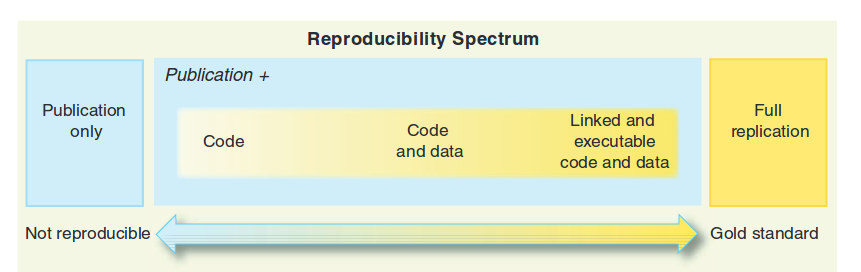
\includegraphics[width=0.8\linewidth]{Reproducible} 

}

\caption{Continuo de reproducibilidad (extraido de Peng 2011)}\label{fig:reproducible}
\end{figure}

En la figura \ref{fig:reproducible} vemos el continuo de replicabilidad
\citep{peng2011reproducible}. En este continuo tenemos el ejemplo de no
reproducibilidad como una publicación sin código. Pasando de menos a más
reproducible por la publicación y el código que genero los resultados y
gráficos; seguido por la publicación, el código y los datos que generan
los resultados y gráficos; y por último código, datos y texto
entrelazados de forma tal que al correr el código obtenemos exactamente
la mismma publicación que leimos.

Esto tiene muchas ventajas, incluyendo el que es más fácil aplicar
exactamente los mismos metodos a otra base de datos, basta poner la
nueva base de datos en el formato que tenía el autor de la primera
publicación y podremos comparar los resultados.

Además en un momento en que la ciencia está basada cada vez más en bases
de datos, se puede poner en el código la recolección y/o muestreo de
datos.

\hypertarget{guardando-nuestro-proyecto-en-github}{%
\section{Guardando nuestro proyecto en
github}\label{guardando-nuestro-proyecto-en-github}}

\hypertarget{que-es-github}{%
\subsection{Que es github?}\label{que-es-github}}

Github es una suerte de dropbox o google drive pensado para la
investigación reproducible, en github cada proyecto es un
\emph{repositorio}. La mayoría de los investigadores que trabajan en
investigación reproducible dejan todo su trabajo documentado en sus
repositorios, lo cual permite interactuar con otros autores.

\hypertarget{creando-un-proyecto-de-github-en-rstudio}{%
\subsection{creando un proyecto de github en
RStudio}\label{creando-un-proyecto-de-github-en-rstudio}}

Para crear un proyecto en github presionamos \textbf{start a project} en
la pagina inicial de nuestra cuenta como vemos en la figura
\ref{fig:Start}

\begin{figure}

{\centering 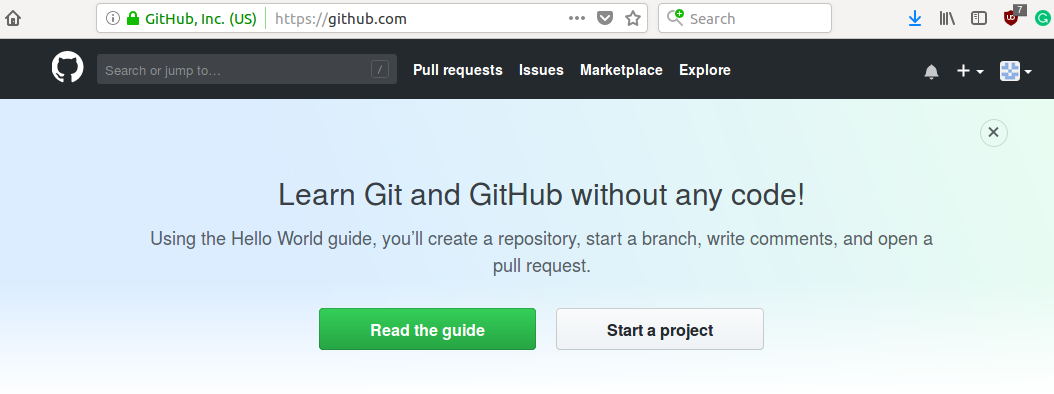
\includegraphics[width=0.8\linewidth]{StartAProject} 

}

\caption{Para empezar un projecto en github, debes presionar Start a project en tu página de inicio}\label{fig:Start}
\end{figure}

Luego crea un nombre unico, y sin cambiar nada más presiona
\textbf{create repository} en el botón verde como vemos en la figura
\ref{fig:Name}.

\begin{figure}

{\centering 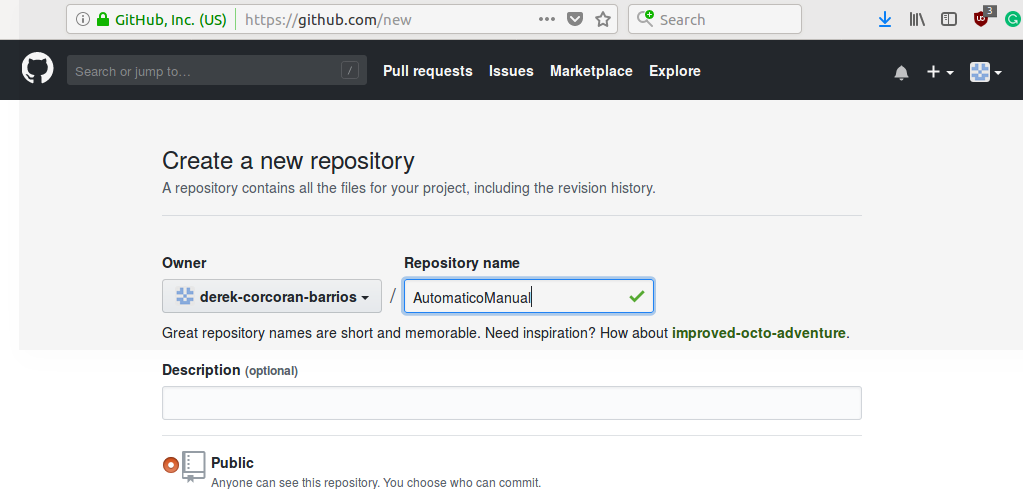
\includegraphics[width=0.8\linewidth]{NombreRepo} 

}

\caption{Crea el nombre de tu repositorio y apreta el boton create repository}\label{fig:Name}
\end{figure}

Esto te llevará a una página donde te aparecera una url de tu nuevo
repositorio como en la figura \ref{fig:ssh}

\begin{figure}

{\centering 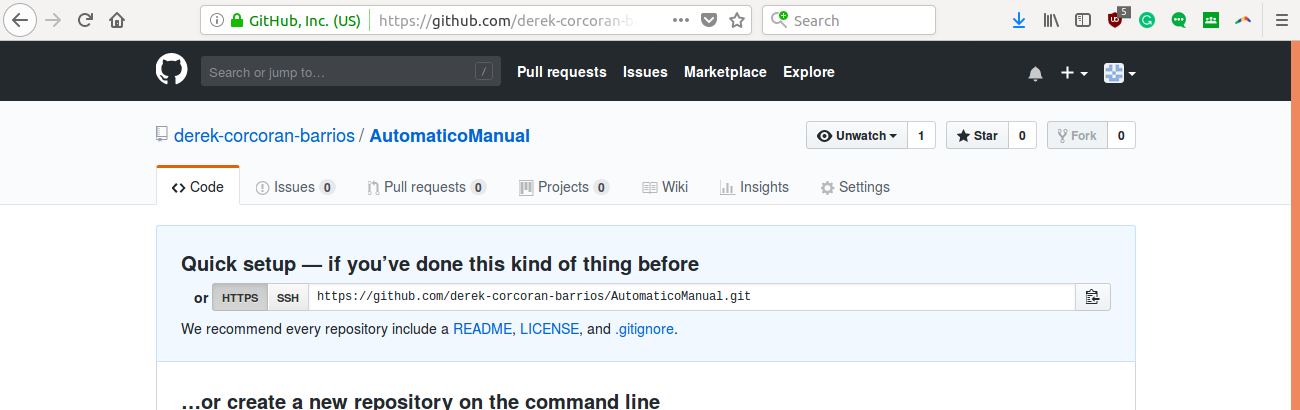
\includegraphics[width=0.8\linewidth]{GitAdress} 

}

\caption{El contenido del cuadro en el cual dice ssh es la url de tu repisitorio}\label{fig:ssh}
\end{figure}

Para incorporar tu proyecto en tu repositorio, lo primero que debes
hacer es generar un proyecto en RStudio, para esto debes ir en el menú
superior de \emph{Rstudio} a \emph{File \textgreater{} New Project
\textgreater{} Git} como se ve en las figuras \ref{fig:NewProject} y
\ref{fig:NewProject}.

\begin{figure}

{\centering 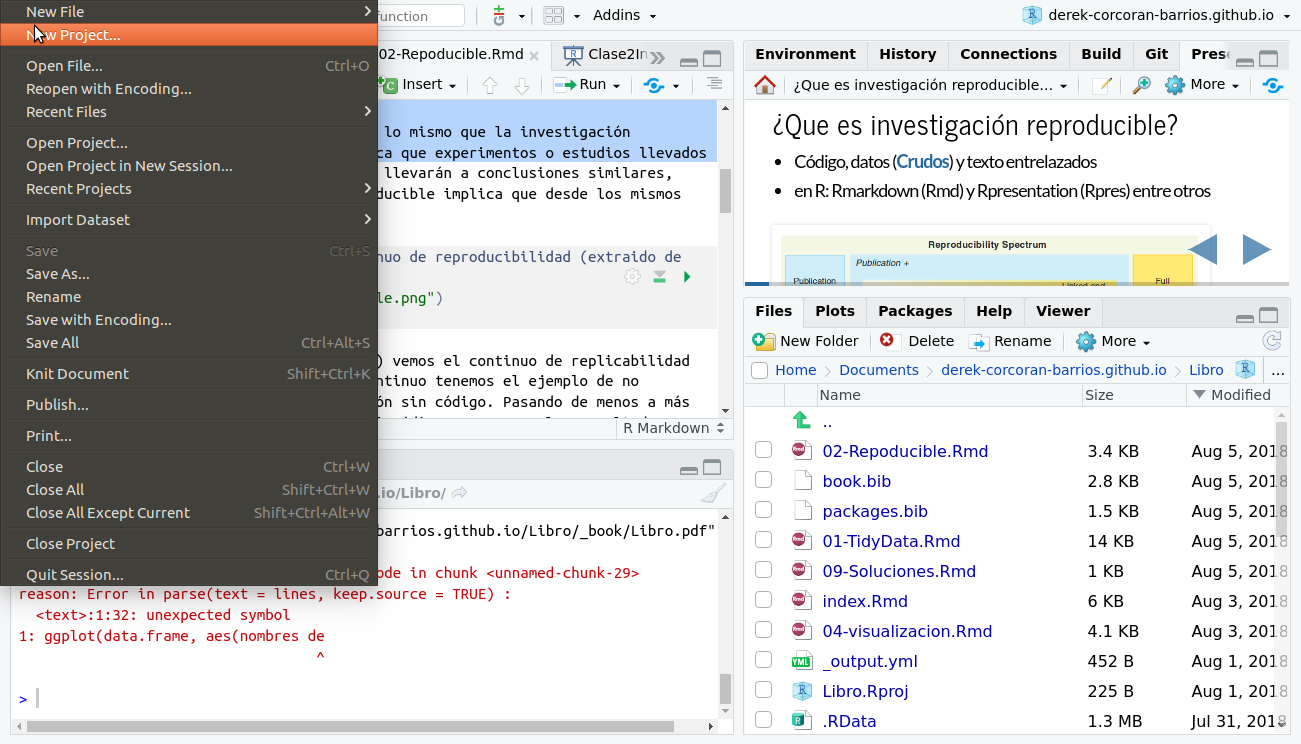
\includegraphics[width=0.8\linewidth]{NewProject} 

}

\caption{Menú para crear un proyecto nuevo}\label{fig:NewProject}
\end{figure}

\begin{figure}

{\centering 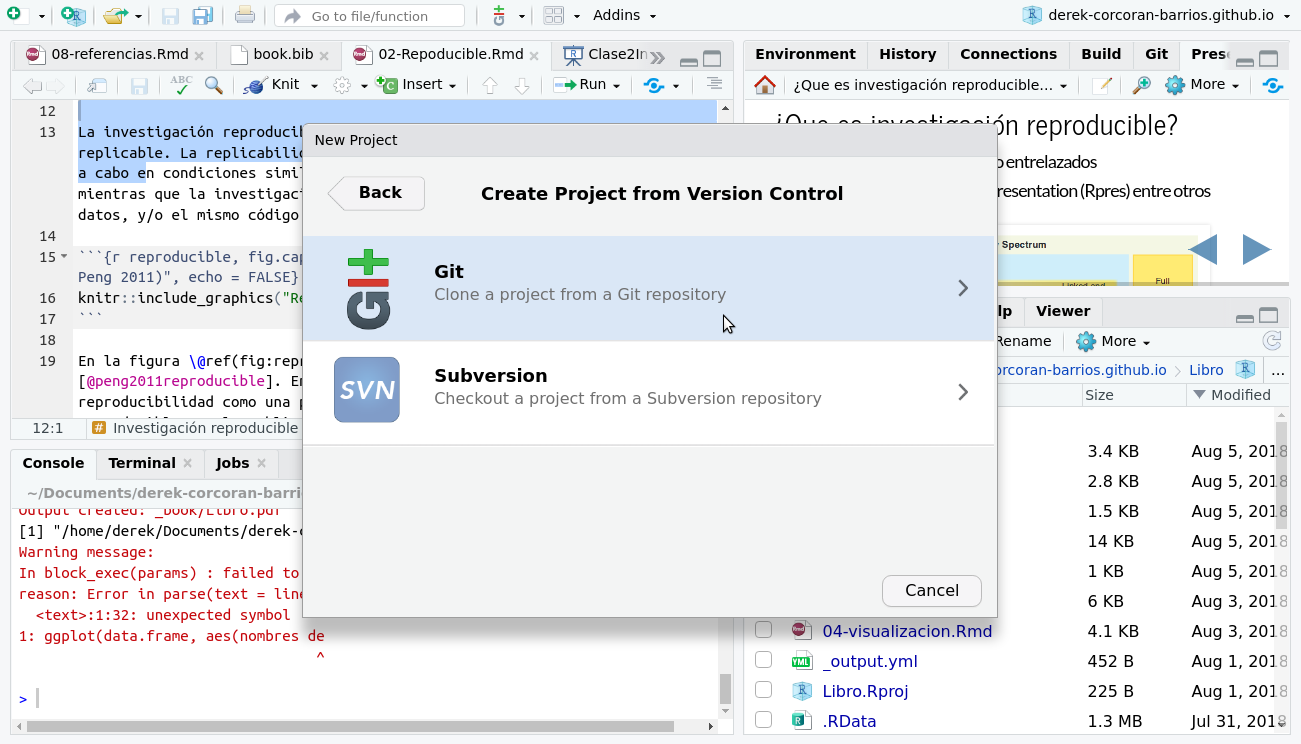
\includegraphics[width=0.8\linewidth]{Git} 

}

\caption{Seleccionar git dentro de las opciones}\label{fig:Git}
\end{figure}

Luego, seleccionar la ubicación del proyecto nuevo y pegar el url que
aparece en la figura \ref{fig:ssh} en el espacio que dice
\textbf{Repository URL:} como muestra en la figura \ref{fig:GitRstudio}.

\begin{figure}

{\centering 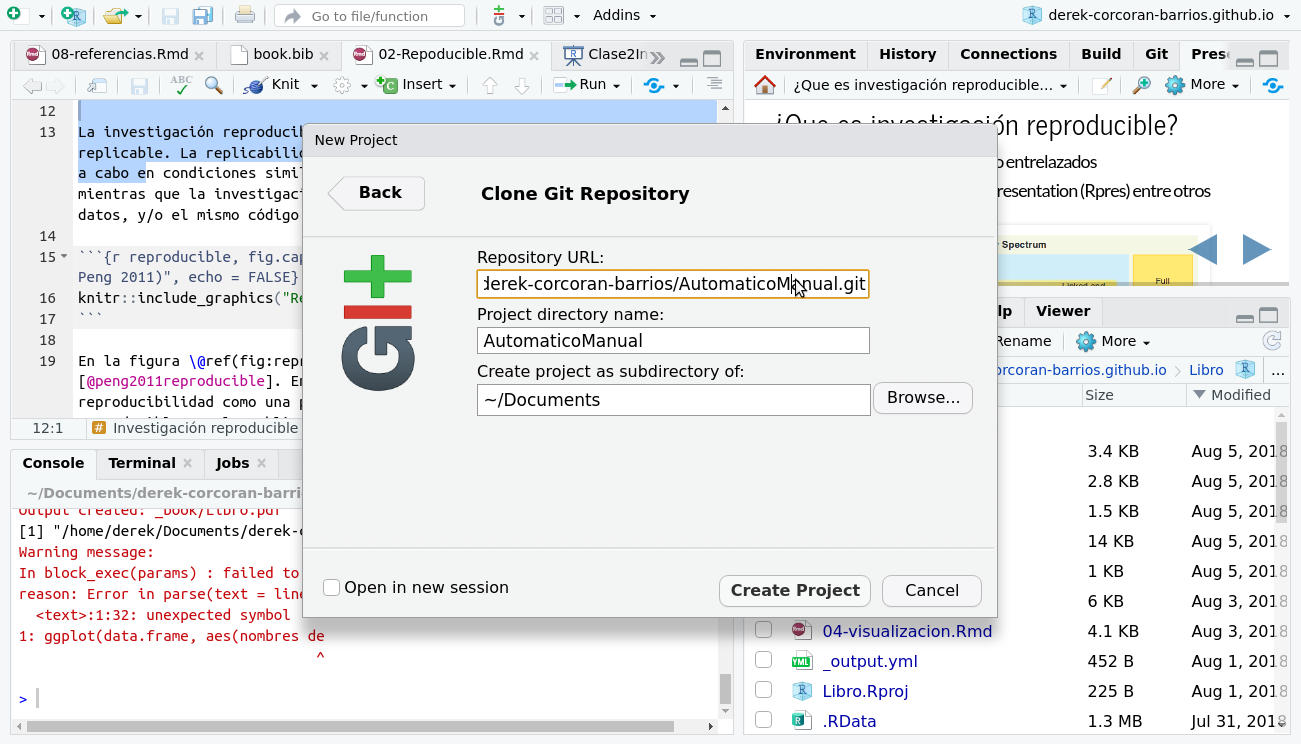
\includegraphics[width=0.8\linewidth]{GitRstudio} 

}

\caption{Pegar el url del repositorio en el cuadro de dialogo Repository URL:}\label{fig:GitRstudio}
\end{figure}

Cuando tu proyecto de R ya este siguiendo los cambios en github, te
aparecera una pestaña git dentro de la ventana superior derecha de tu
sesión de RStudio, tal como vemos en la figura \ref{fig:GitPan}

\begin{figure}

{\centering 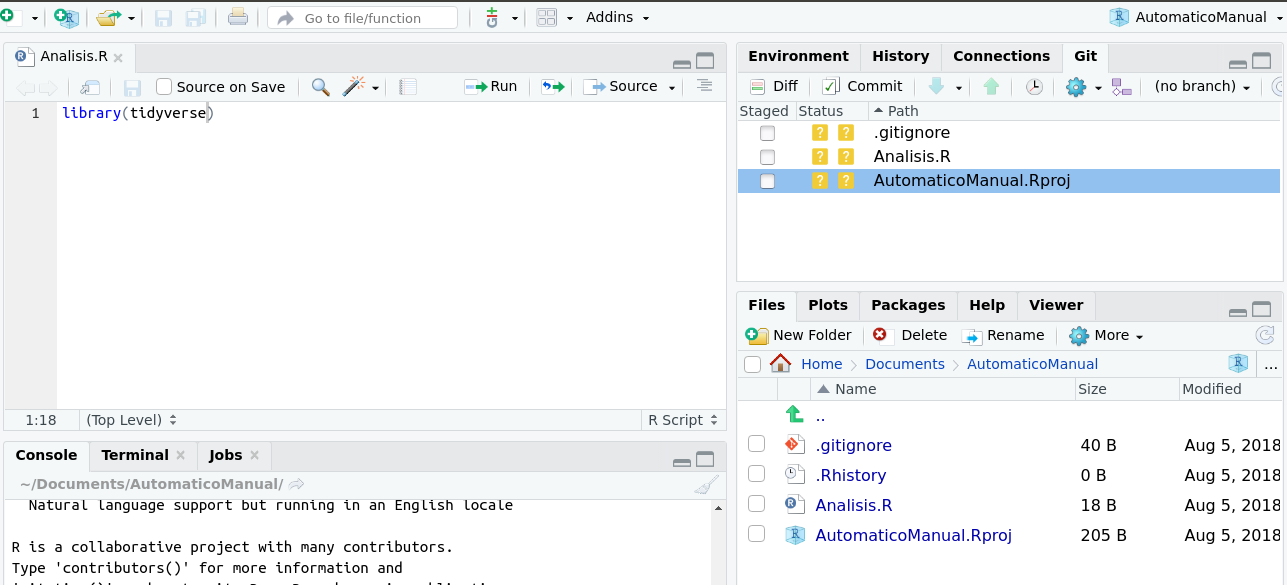
\includegraphics[width=0.8\linewidth]{GitPan} 

}

\caption{Al incluir tu repositorio en tu sesión de Rstudio, aparecera la pestaña git en la ventana superior derecha}\label{fig:GitPan}
\end{figure}

\hypertarget{los-tres-principales-pasos-de-un-repositorio}{%
\subsection{Los tres principales pasos de un
repositorio}\label{los-tres-principales-pasos-de-un-repositorio}}

Github es todo un mundo, con muchas funciones, hay expertos en el uso de
github, pero en este curso, nos enfocaremos en los 3 pasos principales
de un repositorio, \emph{Add}, \emph{commit} y \emph{push}. Para
entender bien que significan cada uno de estos pasos tenemos que
entender que existen dos repositorios en todo momento. Uno local (en tu
computador) u otro remoto (en github.com). Los dos primeros pasos
\emph{Add} y commit, solo generan cambios en tu repositorio local.
Mientras que \emph{push}, salva los cambios al repositorio remoto.

\hypertarget{git-add}{%
\subsubsection{git add}\label{git-add}}

Esta función, es la que agrega archivos a tu repositorio local. Solo
estos archivos serán guardados en github. Cuando tienes bases de datos
mayores a 1 GB no es convenientes guardarlos en github, ya que si bién
te dan repositorios ilimitados, el espacio de cada uno no lo es, en
particular en cuanto a bases de datos. Para adicionar un archivo a tu
repositorio tan solo debes selecionar los archivos en la pestaña git. Al
hacer eso una letra A verde aparecera en vez de los dos signos de
interrogación amarillos, como vemos en la figura \ref{fig:Add}. En este
caso solo adicionamos al repositorio el archivo \emph{Analisis.r} pero
no el resto.

\begin{figure}

{\centering 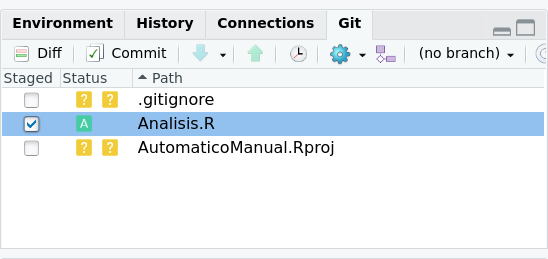
\includegraphics[width=0.8\linewidth]{GitAdd} 

}

\caption{Al incluir tu repositorio en tu sesión de Rstudio, aparecera la pestaña git en la ventana superior derecha}\label{fig:Add}
\end{figure}

\hypertarget{git-commit}{%
\subsubsection{git commit}\label{git-commit}}

Cuando ocupas el comando \emph{commit} estas guardando los cambios de
los archivos que adicionaste, en tu repositorio local. Para hacer esto
en Rstudio, en la misma pestaña de git, debes presionar el botón commit
como vemos en la figura \ref{fig:Commit}.

\begin{figure}

{\centering 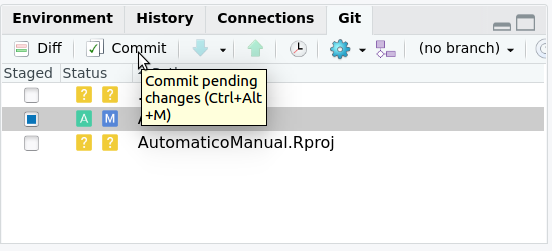
\includegraphics[width=0.8\linewidth]{Commit} 

}

\caption{Para guardar los cambios en tu repositorio apretar commit en la pestaña git de la ventana superior derecha}\label{fig:Commit}
\end{figure}

Al presionar Commit, se abrira una ventana emergente, donde deberás
escribir un mensaje que describa lo que guardaras. Una vez echo eso
presiona commit nuevamente en la ventana emergente como aparece en la
figura \ref{fig:MensajeCommit}.

\begin{figure}

{\centering 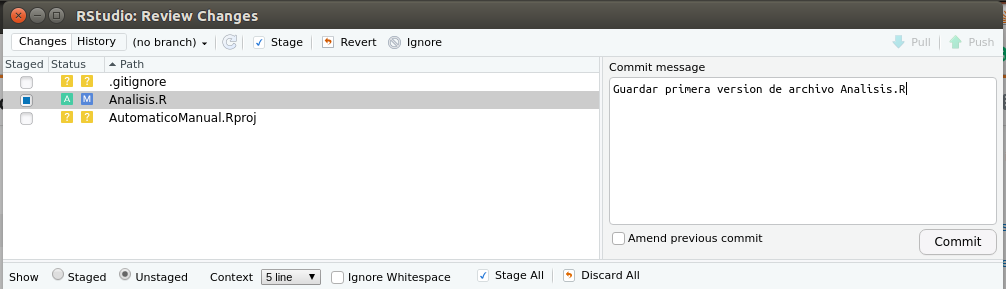
\includegraphics[width=0.8\linewidth]{MensajeCommit} 

}

\caption{Escribir un mensaje que recuerde los cambios que hiciste en la ventana emergente}\label{fig:MensajeCommit}
\end{figure}

\hypertarget{git-push}{%
\subsubsection{git push}\label{git-push}}

Finalmente \emph{push} te permitirá guardar los cambios en tu
repositorio remoto, lo cual asegura tus datos en la nube, y además lo
hace disponible a otros investigadores. Luego de apretar commit en la
ventana emergente (figura \ref{fig:MensajeCommit}), podemos presionar
\emph{push} en la flecha verde de la ventana emergente como se ve el a
figura \ref{fig:push}. Luego se nos pedira nuestro nombre de usuario y
contraseña, y ya podemos revisar que nuestro repositorio esta online
entrando a nuestra sesión de github.

\begin{figure}

{\centering 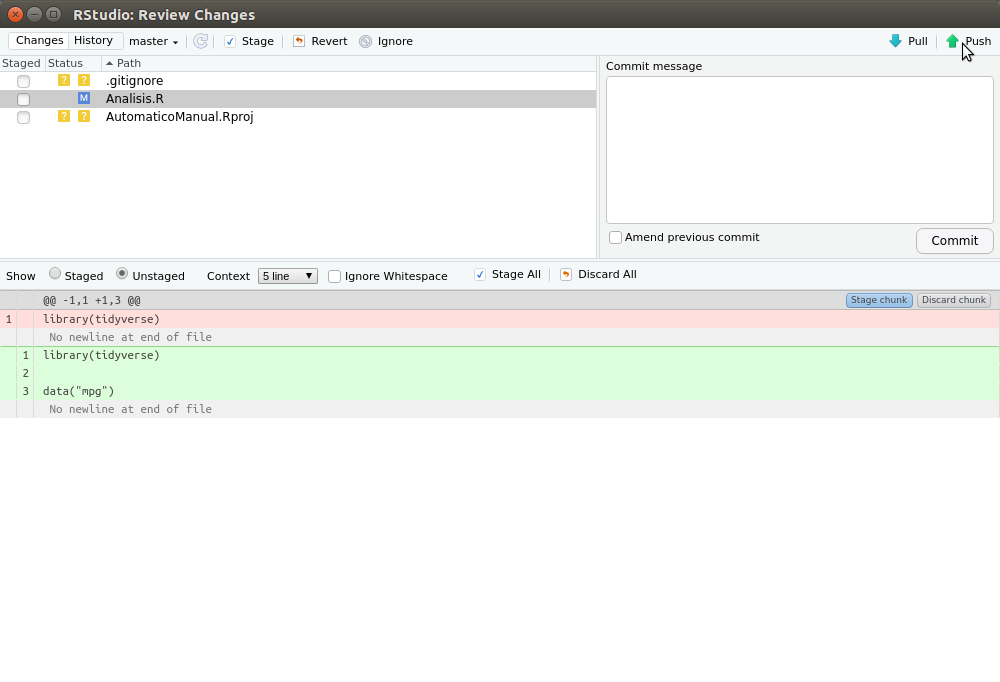
\includegraphics[width=0.8\linewidth]{Push} 

}

\caption{Para guardar en el repositorio remoto apretar push en la ventana emergente}\label{fig:push}
\end{figure}

\hypertarget{reproducibilidad-en-r}{%
\section{Reproducibilidad en R}\label{reproducibilidad-en-r}}

Existen varios paquetes que permiten que hagamos investigación
reproducible en \texttt{R}, pero sin duda los más relevantes son
\emph{rmarkdown} y \emph{knitr}. Ambos paquetes funcionana en conjunto
cuando generamos un archivo \emph{Rmd} (Rmarkdown), en el cual ocupamos
al mismo tiempo texto, código de R y otros elementos para generar un
documento word, pdf, página web, presentación y/o aplicación web (fig
\ref{fig:Rmark}).

\begin{figure}

{\centering 
\includegraphics[width=0.8\linewidth]{Rmark} 

}

\caption{El objetivo de Rmarkdown es el unir código de r con texto y datos para generar un documento reproducible}\label{fig:Rmark}
\end{figure}

\hypertarget{creando-un-rmarkdown}{%
\subsection{Creando un Rmarkdown}\label{creando-un-rmarkdown}}

Para crear un archivo Rmarkdown, simplemente ve a el menu \emph{File
\textgreater{} New file \textgreater{} Rmarkdown} y con eso habrás
creado un nuevo archivo \emph{Rmd}, veremos en momentos algunos de los
elementos más típicos de un arcchivo Rmarkdown.

\hypertarget{markdown}{%
\subsubsection{Markdown}\label{markdown}}

El markdown es la parte del archivo en que simplemente escribimos texto,
aunque tiene algunos detalles para el formato como generar texto en
negrita, cursiva, títulos y subtitulos.

Para hacer que un texto este en \textbf{negrita}, deben ponerlo entre
dos asteriscos \texttt{**negrita**}, para que un texto aparezca en
\emph{cursiva} debe estar entre asteriscos \texttt{*cursiva*}, otros
ejemplos son los titulos de distintos niveles, los cuales se denotan con
distintos números de \texttt{\#}, así los siguientes 4 títulos o
subtitulos:

\hypertarget{subtitulo-1}{%
\section*{subtitulo 1}\label{subtitulo-1}}
\addcontentsline{toc}{section}{subtitulo 1}

\hypertarget{subtitulo-2}{%
\subsection*{subtítulo 2}\label{subtitulo-2}}
\addcontentsline{toc}{subsection}{subtítulo 2}

\hypertarget{subtitulo-3}{%
\subsubsection*{subtítulo 3}\label{subtitulo-3}}
\addcontentsline{toc}{subsubsection}{subtítulo 3}

\hypertarget{subtitulo-4}{%
\paragraph{subtítulo 4}\label{subtitulo-4}}
\addcontentsline{toc}{paragraph}{subtítulo 4}

se vería de la siguiente manera en el código

\begin{Shaded}
\begin{Highlighting}[]
\NormalTok{## subtitulo 1}

\NormalTok{### subtítulo 2}

\NormalTok{#### subtítulo 3}

\NormalTok{##### subtítulo 4}
\end{Highlighting}
\end{Shaded}

\hypertarget{chunks}{%
\subsubsection{Chunks}\label{chunks}}

Los \emph{chunks} son una de las partes más importantes del un
Rmarkdown. En estos es donde se agrega el código de R (u otros lenguajes
de programación). Lo cual permíte que el producto de nuestro código no
sea solo un escrito con resultados pegados, sino que efectivamente
generados en el mismo documento que nuestro escrito, la forma más fácil
de agregar un chunk es apretando el botón de insert chunk en Rstudio,
este boton se encuentra en la ventana superior izquierda de nuestra
sesión de RStudio, tal como se muestra en la figura
\ref{fig:Insertchunk}

\begin{figure}

{\centering 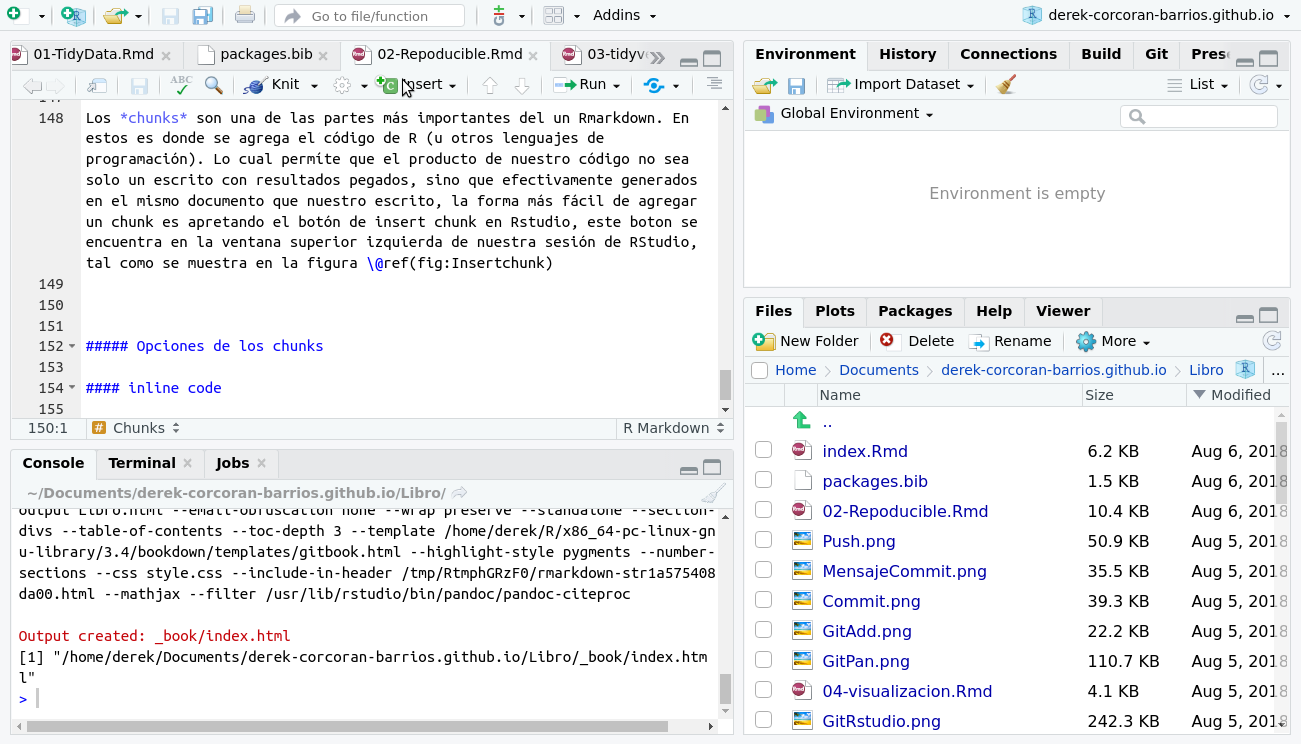
\includegraphics[width=0.8\linewidth]{Insertchunk} 

}

\caption{Al apretar el botón insert chunk, aparecera un espacio en el cuál insertar código}\label{fig:Insertchunk}
\end{figure}

Al apretar este código aparecera un espacio, uno podría agregar un
código como el que aparece a continuación, y vemos a continuación los
resultados.

\begin{Shaded}
\begin{Highlighting}[]
\NormalTok{```\{r\}}
\NormalTok{library(tidyverse)}
\NormalTok{iris %>% group_by(Species) %>% summarize(Petal.Length = mean(Petal.length))}
\NormalTok{```}
\end{Highlighting}
\end{Shaded}

\begin{verbatim}
## # A tibble: 3 x 2
##   Species    Petal.Length
##   <fct>             <dbl>
## 1 setosa             1.46
## 2 versicolor         4.26
## 3 virginica          5.55
\end{verbatim}

\hypertarget{opciones-de-los-chunks}{%
\paragraph{Opciones de los chunks}\label{opciones-de-los-chunks}}

Existen muchas opciones para los chunks, una documentación completa
podemos encontrarle en el siguiente
\href{https://yihui.name/knitr/options/}{link}, pero acá mostraremos los
más comunes:

\begin{itemize}
\tightlist
\item
  \emph{echo} = T o F muestro o no codigo
\item
  \emph{message} = T o F muestra mensajes de paquetes
\item
  \emph{warning} = T o F muestra advertencias
\item
  \emph{eval} = T o F evaluar o no el código
\item
  \emph{cache} = T o F guarda o no el resultado
\end{itemize}

\hypertarget{inline-code}{%
\subsubsection{inline code}\label{inline-code}}

Los \emph{inline codes} son utiles para agregar algún valor en el texto,
como por ejemplo el valor de p, o la media. Para usarlo, se debe poner
un backtick, r, el código en cuestion y otro backtick como se ve a
continuación \texttt{\textasciigrave{}r\ R\_código\textasciigrave{}}. No
podemos poner cualquier cosa en un \emph{inline code}, ya que sólo puede
generar vectores, lo cuál muchas veces requiere de mucha creatividad
para lograr lo que queremos. Por ejemplo si quisieramos poner el
promedio del largo del sépalo de la base da dato \texttt{iris} en un
inline code pondríamos
\texttt{\textasciigrave{}r\ mean(iris\$Sepal.Length)\textasciigrave{}},
lo cual resultaría en 5.8433333. Como en un texto se vería extraño un
número con 7 cifras significativas, querríamos usar ademas la función
\texttt{round}, para que tenga 2 cifras significativas, para eso ponemos
el siguiente inline code
\texttt{\textasciigrave{}r\ round(mean(iris\$Sepal.Length),2)\textasciigrave{}}
que da como resultado 5.84. Esto se puede complejizar más aún, si
queremos trabajar con una tabla resumen, por ejemplo si quisieramos
listar el promedio del tamaño de sépalo usariamos \texttt{summarize} de
\emph{dplyr}, pero esto nos daría como resultado un data.frame, el cual
no aparece si intentamos hacer un inline code. Partamos por ver como se
vería el código donde obtuvieramos la media del tamaño del sépalo.

\begin{Shaded}
\begin{Highlighting}[]
\NormalTok{iris }\OperatorTok\StringTok{ }\KeywordTok{group_by}\NormalTok{(Species) }\OperatorTok\StringTok{ }\KeywordTok{summarize}\NormalTok{(}\DataTypeTok{Mean =} \KeywordTok{mean}\NormalTok{(Sepal.Length))}
\end{Highlighting}
\end{Shaded}

El resultado de ese código lo veríamos \ref{tab:SummarySepaltab}

\begin{table}

\caption{\label{tab:SummarySepaltab}Resumen del promedio del largo de sépalo de las flores del genero Iris.}
\centering
\begin{tabular}[t]{lr}
\toprule
Species & Mean\\
\midrule
setosa & 5.006\\
versicolor & 5.936\\
virginica & 6.588\\
\bottomrule
\end{tabular}
\end{table}

Para sacar de este data frame el vector de la média podríamos
subsetearlo con el signo \texttt{\$}, entonces si queremos sacar como
vector la columna \emph{Mean}, del data frame que creamos haríamos lo
siguiente
\texttt{\textasciigrave{}r\ (iris\ \%\textgreater{}\%\ group\_by(Species)\ \%\textgreater{}\%\ summarize(Mean\ =\ mean(Sepal.Length)))\$Mean\textasciigrave{}},
lo cual daría como resultado 5.006, 5.936, 6.588.

\hypertarget{tablas-en-rmarkdown}{%
\subsubsection{Tablas en Rmarkdown}\label{tablas-en-rmarkdown}}

la función más típica para generar tablas en un archivo \emph{rmd} es
\texttt{kable} del paquete \emph{knitr}, que en su forma más simple se
incluye un dataframe adentro y obtenemos una tabla, además de esto,
podemos agregar algunos parametros como \emph{caption}, que nos permite
poner un título a la tabla o \emph{row.names}, que si se pone como se ve
en el código (FALSE) no mostrará en la tabla los nombres de las filas,
tal como se ve en la tabla \ref{tab:SummaryMeans}.

\begin{Shaded}
\begin{Highlighting}[]
\NormalTok{DF <-}\StringTok{ }\NormalTok{iris }\OperatorTok\StringTok{ }\KeywordTok{group_by}\NormalTok{(Species) }\OperatorTok\StringTok{ }\KeywordTok{summarize_all}\NormalTok{(mean)}
\KeywordTok{kable}\NormalTok{(DF, }\DataTypeTok{caption =} \StringTok{"Promedio por especie de todas las variables de la base de datos iris."}\NormalTok{, }
    \DataTypeTok{row.names =} \OtherTok{FALSE}\NormalTok{)}
\end{Highlighting}
\end{Shaded}

\begin{table}

\caption{\label{tab:SummaryMeans}Promedio por especie de todas las variables de la base de datos iris.}
\centering
\begin{tabular}[t]{lrrrr}
\toprule
Species & Sepal.Length & Sepal.Width & Petal.Length & Petal.Width\\
\midrule
setosa & 5.006 & 3.428 & 1.462 & 0.246\\
versicolor & 5.936 & 2.770 & 4.260 & 1.326\\
virginica & 6.588 & 2.974 & 5.552 & 2.026\\
\bottomrule
\end{tabular}
\end{table}

\hypertarget{tidyverso}{%
\chapter{El Tidyverso}\label{tidyverso}}

We describe our methods in this chapter.

\hypertarget{visualizacion}{%
\chapter{Visualización de datos}\label{visualizacion}}

En este capítulo aprenderemos a usar el paquete \emph{ggplot2}
\citep{Wickhamggplot}, parte del paquete \emph{tidyverse}
\citep{Wickhamtidyverse}.

\hypertarget{el-esqueleto}{%
\section{El esqueleto}\label{el-esqueleto}}

El esqueleto de una visualización usando \emph{ggplot2} es la siguiente

\begin{Shaded}
\begin{Highlighting}[]
\KeywordTok{ggplot}\NormalTok{(data.frame, }\KeywordTok{aes}\NormalTok{(nombres_de_columna)) }\OperatorTok{+}\StringTok{ }\KeywordTok{geom_algo}\NormalTok{(argumentos, }
    \KeywordTok{aes}\NormalTok{(columnas)) }\OperatorTok{+}\StringTok{ }\KeywordTok{theme_algo}\NormalTok{()}
\end{Highlighting}
\end{Shaded}

Como ejemplo para discutir usaremos el siguiente código que genera la
figura \ref{fig:ejemplo1-ggplot}:

\begin{Shaded}
\begin{Highlighting}[]
\KeywordTok{library}\NormalTok{(tidyverse)}
\KeywordTok{data}\NormalTok{(}\StringTok{"diamonds"}\NormalTok{)}
\KeywordTok{ggplot}\NormalTok{(diamonds, }\KeywordTok{aes}\NormalTok{(}\DataTypeTok{x =}\NormalTok{ carat, }\DataTypeTok{y=}\NormalTok{price)) }\OperatorTok{+}\StringTok{ }\KeywordTok{geom_point}\NormalTok{(}\KeywordTok{aes}\NormalTok{(}\DataTypeTok{color =}\NormalTok{ cut)) }\OperatorTok{+}\StringTok{ }\KeywordTok{theme_classic}\NormalTok{()}
\end{Highlighting}
\end{Shaded}

\begin{figure}

{\centering 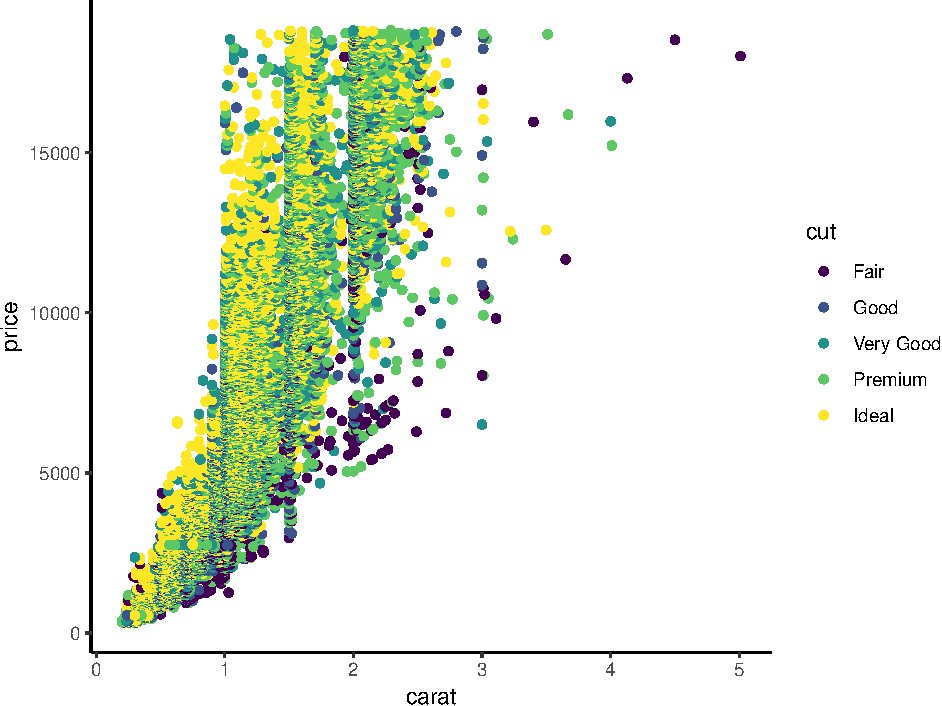
\includegraphics[width=0.8\linewidth]{Libro_files/figure-latex/ejemplo1-ggplot-1} 

}

\caption{Gráfico en el cual gráficamos los quilates de diamantes versus su precio, con el corte del diamante representado por el color}\label{fig:ejemplo1-ggplot}
\end{figure}

En este caso general, lo primero que ponemos después de ggplot es el
data.frame desde el cuál graficaremos algo, en el ejemplo de la figura
\ref{fig:ejemplo1-ggplot} usamos la base de datos \emph{diamonds} del
paquete \emph{ggplot2} \citep{Wickhamggplot}. Luego dentro de
\texttt{aes} ponemos las columnas que graficaremos como \emph{x} y/o
\emph{y}, en nuestro ejemplo dentro de aes ponemos como eje \emph{x} los
kilates de los diamantes (caret) y como \emph{y} el precio de los mismos
(price). La necesidad de poner \texttt{aes} en ggplot2 (algo que no
había sido necesario cuando usamos \emph{dplyr} o \emph{tidyr}) es que
ggplot2 es el paquete mas antiguo del \emph{tidyverse}.

\hypertarget{geom_algo}{%
\section{geom\_algo}\label{geom_algo}}

Luego de especificar una base de datos, esto viene seguido de un
\texttt{geom\_algo}, esto nos indicará que tipo de gráfico usaremos,
estos pueden ser combinados como veremos en ejemplos futuros

\hypertarget{una-variable-categorica-una-continua}{%
\subsection{Una variable categórica una
continua}\label{una-variable-categorica-una-continua}}

Primero veremos algunos de los \emph{geom} que podemos utilizar con una
variable categórica y una continua

\hypertarget{geom_boxplot}{%
\subsubsection{geom\_boxplot}\label{geom_boxplot}}

En la figura \ref{fig:boxplot}, generado a partir del código a
continuacón con la base de datos iris presente en \texttt{R}
\citep{anderson1935irises}.

\begin{Shaded}
\begin{Highlighting}[]
\KeywordTok{data}\NormalTok{(}\StringTok{"iris"}\NormalTok{)}
\KeywordTok{ggplot}\NormalTok{(iris, }\KeywordTok{aes}\NormalTok{(}\DataTypeTok{x =}\NormalTok{ Species, }\DataTypeTok{y =}\NormalTok{ Sepal.Length)) }\OperatorTok{+}\StringTok{ }\KeywordTok{geom_boxplot}\NormalTok{()}
\end{Highlighting}
\end{Shaded}

\begin{figure}

{\centering 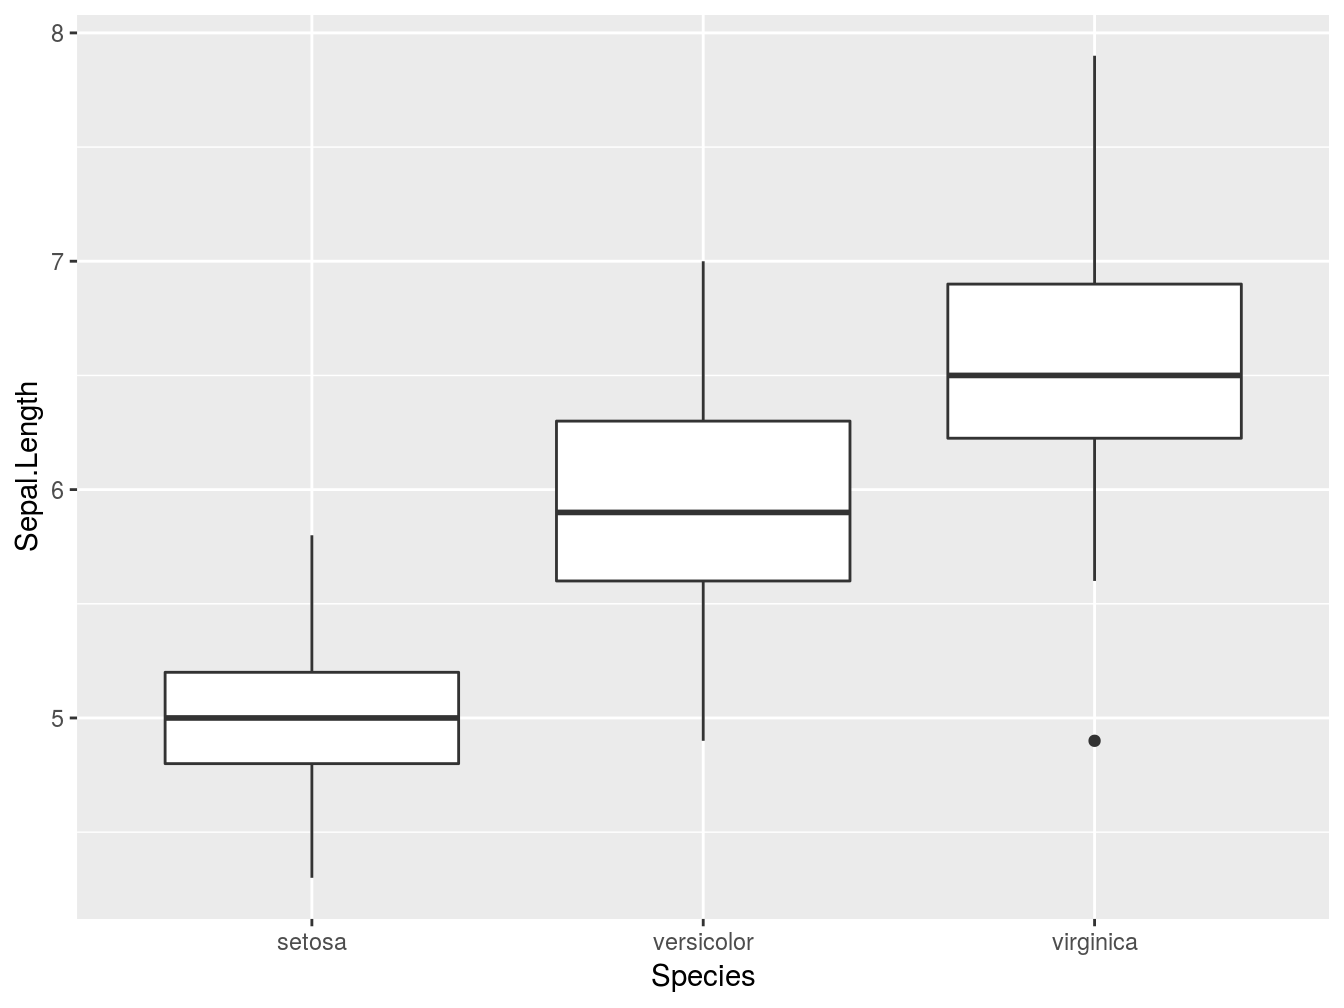
\includegraphics[width=0.8\linewidth]{Libro_files/figure-latex/boxplot-1} 

}

\caption{Boxplot que representa los largos del sépalo de tres especies del género Iris}\label{fig:boxplot}
\end{figure}

Los boxplots muestran una linea gruesa central (la mediana), una caja,
que delimita el primer y tercer cuartil, y los bigotes, los cuales se
extienden hasta los valores extremos. A menos que estos esten por sobre
1.5 veces la distance entre el primer y tercer cuartil, en cuyo caso se
consideran outlyers, y estos son representados por puntos. En la figura
\ref{fig:boxplot}, solo \emph{Iris virginica} presenta un outlayer en
cuanto a las medidas del largo del sepalo.

Los boxplots, como todos los gráficos pueden ser personalizados usando
otros argumentos, los cuales son detallados en la sección
\ref{argumentos}, pero en los ejemplos que mostraremos en esta sección
los iremos introduciendo de a poco. Si quisieramos por ejemplo que el
color de las cajas del \emph{boxplot} fuera deacuerdo a la especie,
cambiamos el llenado (\textbf{fill}) de la caja, como vemos en el
siguiente ejemplo y figura \ref{fig:boxplot2}

\begin{Shaded}
\begin{Highlighting}[]
\KeywordTok{ggplot}\NormalTok{(iris, }\KeywordTok{aes}\NormalTok{(}\DataTypeTok{x =}\NormalTok{ Species, }\DataTypeTok{y =}\NormalTok{ Sepal.Length)) }\OperatorTok{+}\StringTok{ }\KeywordTok{geom_boxplot}\NormalTok{(}\KeywordTok{aes}\NormalTok{(}\DataTypeTok{fill =}\NormalTok{ Species))}
\end{Highlighting}
\end{Shaded}

\begin{figure}

{\centering 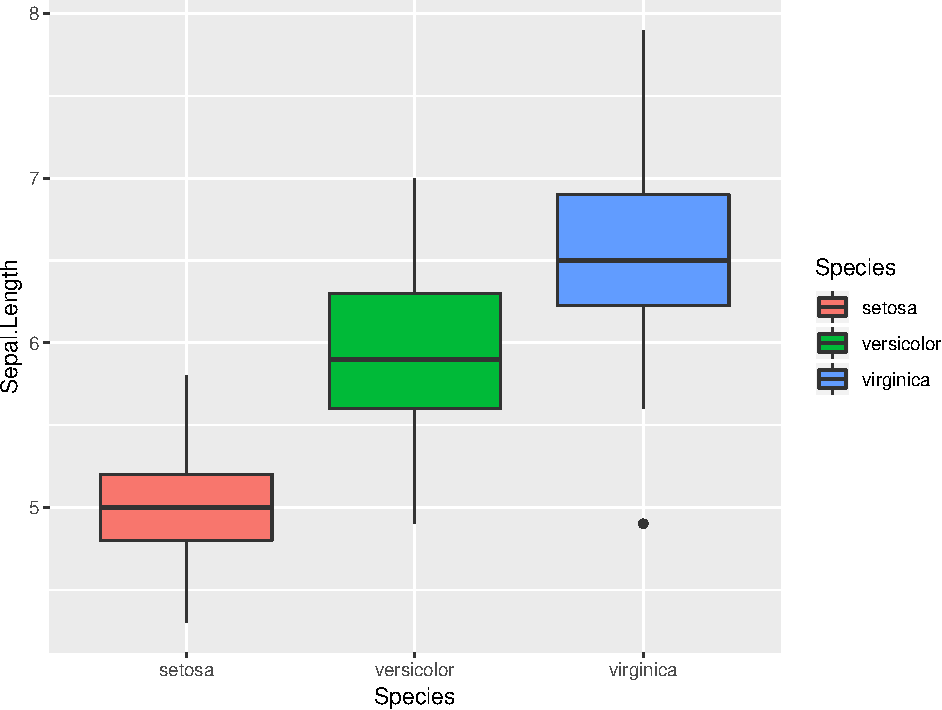
\includegraphics[width=0.8\linewidth]{Libro_files/figure-latex/boxplot2-1} 

}

\caption{Boxplot que representa los largos del sépalo de tres especies del género Iris, en este caso el color de la caja representa la especie}\label{fig:boxplot2}
\end{figure}

Dos cosas a notar en este ejemplo, por un lado la leyenda se genera de
forma automática, y por otro lado, vemos que es necesario poner
\emph{Species} dentro de \texttt{aes}, esto es debido a que Species es
una columna y como se explicó al principio de este capítulo, todas las
columnas deben ser incuidas dentro de la función \texttt{aes} para poder
ser referenciadas.

\hypertarget{geom_jitter}{%
\subsubsection{geom\_jitter}\label{geom_jitter}}

\begin{Shaded}
\begin{Highlighting}[]
\KeywordTok{ggplot}\NormalTok{(iris, }\KeywordTok{aes}\NormalTok{(}\DataTypeTok{x =}\NormalTok{ Species, }\DataTypeTok{y =}\NormalTok{ Sepal.Length)) }\OperatorTok{+}\StringTok{ }\KeywordTok{geom_jitter}\NormalTok{(}\KeywordTok{aes}\NormalTok{(}\DataTypeTok{color =}\NormalTok{ Species))}
\end{Highlighting}
\end{Shaded}

\begin{figure}

{\centering 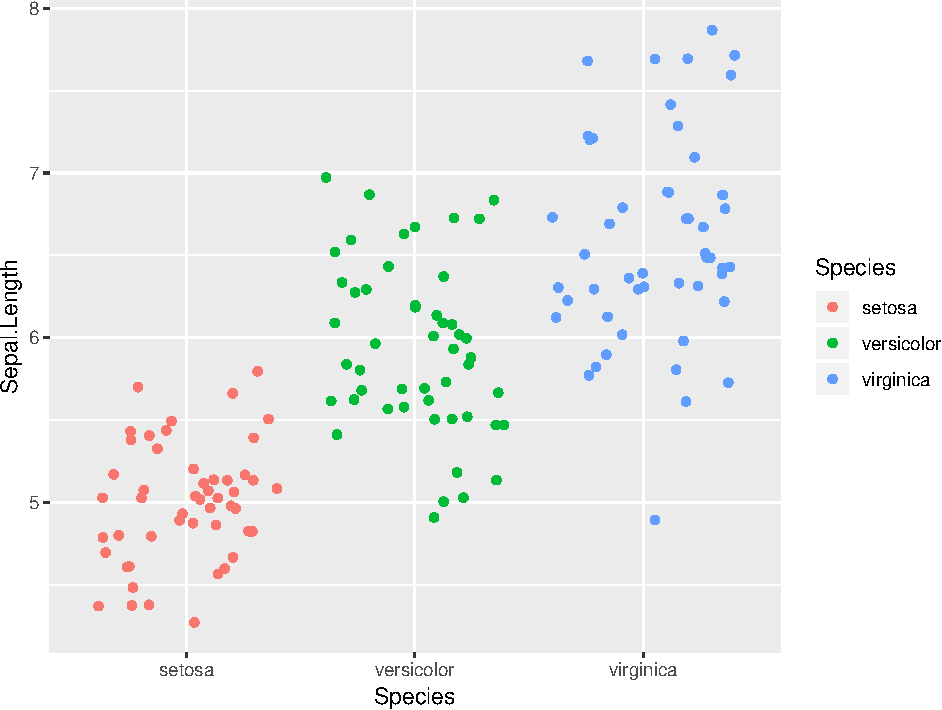
\includegraphics[width=0.8\linewidth]{Libro_files/figure-latex/jitter-1} 

}

\caption{Boxplot que representa los largos del sépalo de tres especies del género Iris, en este caso el color de la caja representa la especie}\label{fig:jitter}
\end{figure}

\hypertarget{argumentos}{%
\section{Argumentos}\label{argumentos}}

\hypertarget{modelos}{%
\chapter{Modelos en R}\label{modelos}}

We have finished a nice book.

\hypertarget{loops}{%
\chapter{Loops (purrr) y bibliografía (rticles)}\label{loops}}

\hypertarget{presentacion}{%
\chapter{Presentaciones en R}\label{presentacion}}

\hypertarget{soluciones}{%
\chapter{Soluciones a problemas}\label{soluciones}}

Todos los problemas en programación tienen más de una forma de llegar a
ellos, es por esto que las soluciones acá mostradas deben tomarse solo
como una referencia, y revisar si el resultado final de tu código
(aunque sea distinto de este), sea igual al que presentamos.

\hypertarget{capitulo-1}{%
\section{Capítulo 1}\label{capitulo-1}}

\hypertarget{ejercicio-1-1}{%
\subsection{Ejercicio 1}\label{ejercicio-1-1}}

Algunas posibles soluciones:

\begin{Shaded}
\begin{Highlighting}[]
\NormalTok{storms }\OperatorTok\StringTok{ }\KeywordTok{filter}\NormalTok{(status }\OperatorTok{==}\StringTok{ "hurricane"}\NormalTok{) }\OperatorTok\StringTok{ }\KeywordTok{select}\NormalTok{(year, wind, }
\NormalTok{    hu_diameter) }\OperatorTok\StringTok{ }\KeywordTok{group_by}\NormalTok{(year) }\OperatorTok\StringTok{ }\KeywordTok{summarize_all}\NormalTok{(mean)}
\end{Highlighting}
\end{Shaded}

\begin{Shaded}
\begin{Highlighting}[]
\NormalTok{storms }\OperatorTok\StringTok{ }\KeywordTok{filter}\NormalTok{(status }\OperatorTok{==}\StringTok{ "hurricane"} \OperatorTok{&}\StringTok{ }\OperatorTok{!}\KeywordTok{is.na}\NormalTok{(hu_diameter)) }\OperatorTok\StringTok{ }
\StringTok{    }\KeywordTok{select}\NormalTok{(year, wind, hu_diameter) }\OperatorTok\StringTok{ }\KeywordTok{group_by}\NormalTok{(year) }\OperatorTok\StringTok{ }\KeywordTok{summarize_all}\NormalTok{(mean)}
\end{Highlighting}
\end{Shaded}

\begin{Shaded}
\begin{Highlighting}[]
\NormalTok{storms }\OperatorTok\StringTok{ }\KeywordTok{filter}\NormalTok{(status }\OperatorTok{==}\StringTok{ "hurricane"}\NormalTok{) }\OperatorTok\StringTok{ }\KeywordTok{select}\NormalTok{(year, wind, }
\NormalTok{    hu_diameter) }\OperatorTok\StringTok{ }\KeywordTok{group_by}\NormalTok{(year) }\OperatorTok\StringTok{ }\KeywordTok{summarize_all}\NormalTok{(}\KeywordTok{funs}\NormalTok{(mean), }
    \DataTypeTok{na.rm =} \OtherTok{TRUE}\NormalTok{)}
\end{Highlighting}
\end{Shaded}

\hypertarget{ejercicio-2-1}{%
\subsection{Ejercicio 2}\label{ejercicio-2-1}}

Una de las soluciones posibles:

\begin{Shaded}
\begin{Highlighting}[]
\NormalTok{Solution <-}\StringTok{ }\NormalTok{mpg }\OperatorTok\StringTok{ }\KeywordTok{filter}\NormalTok{(year }\OperatorTok{>}\StringTok{ }\DecValTok{2004} \OperatorTok{&}\StringTok{ }\NormalTok{class }\OperatorTok{==}\StringTok{ "compact"}\NormalTok{) }\OperatorTok\StringTok{ }
\StringTok{    }\KeywordTok{mutate}\NormalTok{(}\DataTypeTok{kpl =}\NormalTok{ (cty }\OperatorTok{*}\StringTok{ }\FloatTok{1.609}\NormalTok{)}\OperatorTok{/}\FloatTok{3.78541}\NormalTok{)}
\end{Highlighting}
\end{Shaded}

\bibliography{book.bib,packages.bib}


\end{document}
